%%
%% THESIS/DISSERTATION TEMPLATE FOR THE UNIVERSITY OF ALABAMA.
%%
%% This example is written by Paul Kilgo. It highlights all the (few) features
%% of uathesis.cls
%% Modified by Yuanyuan Song(2014) for the requirements of Ph.D thesis.

%% Use one of the following if writing a thesis/dissertation.
% \documentclass[thesis]{uathesis}
\documentclass[dissertation]{uathesis}
\graphicspath{{figs/}}
%% Basic packages you'll probably want to use.
\usepackage{graphicx}                 %% For using \includegraphics{}
\usepackage{cite}                     %% For sorting/collapsing citations.
\usepackage{color}                    %% For colors used in listings.
\usepackage{listings}                 %% Code listings (for engineers)
\usepackage{lipsum}
\usepackage[section]{placeins}
\usepackage{calc}
\usepackage{amsmath,array}
\usepackage{epstopdf}
\usepackage{morefloats}
\usepackage{subfig}
\usepackage{graphicx}
\usepackage[countmax]{subfloat}
%\usepackage[]{mcode}                 %% For including programming code
\usepackage{setspace}
%\usepackage{breqn}
%% Includes
%\input{inc/glossary.tex} %nomenclature
% TODO: If you have any special commands defined, include them here.

%%%%%%%%%%%%%%%%%%%%%%%%%%%New commands%%%%%%%%%%%%%%%%%%%%%%%%
\newcommand\Real{\mbox{Re}} % cf plain TeX's \Re and Reynolds number
\newcommand\Imag{\mbox{Im}} % cf plain TeX's \Im
\newcommand\Rey{\mbox{\textit{Re}}}  % Reynolds number
\newcommand\Ma{\mbox{\textit{Ma}}}  % Marangoni number
\newcommand\C{\mbox{\textit{C}}}  % Surfactant concentration
\newcommand\G{\mbox{\textit{G}}}
%\newcommand\A21{\mbox{\textit{\left[A\right]^2_1}}} % For the example of [A]^2_1
\newcommand\Ca{\mbox{\textit{Ca}}}  % Modified Capillary number
\newcommand\Or{\mbox{\textit{O}}}
\newcommand\slsA{\mathsfbi{A}} % for sans serif bold-sloping Q
\newcommand\etal{\mbox{\textit{et al.}}}
\newcommand\eps{\epsilon}
\newcommand{\pa}[2]{\frac{\partial #1}{\partial #2}}
\newcommand{\de}[2]{\frac{\mathrm{d} #1}{\mathrm{d} #2}}
\newcommand\Rsm{R_{sm}}
\newcommand\Rmg{R_{mg}}
\newcommand\Rw{R_{ws}}
\newcommand\Rwi{\overline{\Rw}}
\newcommand\Rsmi{\overline{\Rsm}}
\newcommand\Rmgi{\overline{\Rmg}}
\newcommand\Rj{{R_{j}}}
\newcommand\Rjz{{R_{j}}_z}
\newcommand\Rjzz{{R_{j}}_{zz}}
\newcommand\Rjzs{{R^\ast_{j}}_{z^\ast}}
\newcommand\Rjzzs{{R^\ast_{j}}_{z^\ast z^\ast}}
\newcommand\Rwz{{R_{ws}}_z}
\newcommand\Rsmz{{R_{sm}}_z}
\newcommand\Rmgz{{R_{mg}}_z}
\newcommand\Rwzz{{R_{ws}}_{zz}}
\newcommand\Rsmzz{{R_{sm}}_{zz}}
\newcommand\Rmgzz{{R_{mg}}_{zz}}
\newcommand\Rwt{{R_{ws}}_t}
\newcommand\Rsmt{{R_{sm}}_t}
\newcommand\Rmgt{{R_{mg}}_t}
\newcommand\ez{\eta_z}
\newcommand\az{\alpha_z}
\newcommand\bz{\beta_z}
\newcommand\gz{\mbox{\textit{G}}_z}
\newcommand\ezz{\eta_{zz}}
\newcommand\azz{\alpha_{zz}}
\newcommand\bzz{\beta_{zz}}
\newcommand\gzz{\mbox{\textit{G}}_{zz}}
\newcommand\ezzz{\eta_{zzz}}
\newcommand\azzz{\alpha_{zzz}}
\newcommand\bzzz{\beta_{zzz}}
\newcommand\gzzz{\mbox{\textit{G}}_{zzz}}
\newcommand\ezzzz{\eta_{zzz}}
\newcommand\azzzz{\alpha_{zzzz}}
\newcommand\bzzzz{\beta_{zzzz}}
\newcommand\gzzzz{\mbox{\textit{G}}_{zzzz}}
\newcommand\et{\eta_t}
\newcommand\at{\alpha_t}
\newcommand\bt{\beta_t}
\newcommand\gt{\mbox{\textit{G}}_t}
\newcommand\Rmgif{\Rmgi^4}
\newcommand\Rmgit{\Rmgi^2}
\newcommand\Rsmif{\Rmgi^4}
\newcommand\Rsmit{\Rsmi^2}


%%%%%%%%%%%%%%%%%%%%%%%%%%%%%%%%%%%%%%%%%%%%%%%%%%%%%%%%%%%%%%%%%


%% Required parameters (these default to undefined)
\author{Sheik Ahmed Ullah}       %% Your name!
\adviser{Shan Zhao}      %% Your adviser/committee chair!

%% The people on your committee.
%% Use \and to break them up between lines.
\committee{
  DAVID HALPERN \and
  BRENDAN AMES \and
  MUHAMMAD A. R. SHARIF \and
  MOJDEH RASOULZADEH
}

%% Note the use of \and to create line breaks and the
%% inverted pyramid style requested by the graduate school.

\title{A new ADI method for the Poisson-Boltzmann equation with \protect\\ a two-component regularization}

\degree{Doctor of Philosophy}   %% Change to suit your degree.
\department{Mathematics}        %% Change to suit your department.

%% These are body text paragraphs to be placed in the front matter.
\abstract{
The Poisson Boltzmann equation (PBE) is a well-established implicit solvent continuum model for the electrostatic analysis of solvated biomolecules. The solution for the nonlinear PBE is still a challenge due to its strong singularity by the source terms, dielectrically distinct regions, and exponential nonlinear terms. In this dissertation, a new alternating direction implicit method (ADI) is proposed for solving the nonlinear PBE using a two-component regularization. This scheme inherits all the advantages of the two-component regularization and the time-dependent PBE with ADI method while possess a novel approach to combine them. A modified version of the one-dimensional ghost fluid method (GFM) has been introduced to incorporate the nonzero jump condition into a new ADI method to propose GFM-ADI method. It produced better results in terms of  spatial accuracy and stability compared to the previous ADI method and simpler to implement by circumventing the work necessary to apply the MIB method with the regularization for a 3D problem. Moreover, the stability of the GFM-ADI method has been significantly improved in comparing with the non-regularized ADI method, so that stable protein simulations can be carried out with a pretty large time step size. Two locally one-dimensional (LOD) methods have also been developed for the time-dependent regularized PBE, which are unconditionally stable.  
%To continue the  search for more stable methods this modified GFM method and Locally One Dimensional (LOD) method has been combined similarly with Implicit Euler method and Crank-Nicolson method two propose GFM-LODCN and GFM-ODIE method. 
%{\color{red}Though this scheme can use larger time increments than the previous ADI method, it still blows up for large time increments. Later to address this issue with the stability, Locally One Dimensional (LOD) method has been used to replace the ADI method as the operator splitting part.} 
Finally, for numerical validation, we have evaluated the solvation free energy for a collection of 24 proteins with various sizes and the salt effect on the protein-protein binding energy of the complex 1beb.
}

\dedication{
To my loving parents and all the teachers in my life who inspired, helped and cared for me to pursue my interests in mathematics.  
}

\acknowledgments{
I wish to express my most sincere gratitude and appreciation to Professor Shan Zhao for his guidance, patience and encouragement. Without his help it would have been difficult for me to be focused to the right direction with all the patience and perseverance necessary before scholarly success. He has always been by my side as a local guardian and it meant a lot to me.  His funding from the NSF grant DMS-1812930 titled "{\it A regularized Poisson Boltzmann model for fast computation of the ensemble average polar solvation energy}" was also a great support for the last part of my Ph. D. program. 

I would also like to express my gratitude toward my committee members for their time and support: the external member from the Department of Aerospace Engineering and Mechanics at the University of Alabama, Dr. Muhammad Ali Rob Sharif and the local members from the Department of Mathematics at the University of Alabama, Dr. Brendan Ames, Dr. Mojdeh Rasoulzadeh and Professor David Halpern. I want to specially thank Professor Halpern for his help and guidance to get my access to the High Performance Computing facility from UAHPC and introducing me to the Summer School at the MSRI, UC Berkeley. I wish to express my indebtedness to Professor David Cruz-Uribe for his continuous support to arrange travel funds from the Graduate School, and the College of Arts and Sciences. 

I want to take this occasion to thank Dr. Weihua Geng from the Southern Methodists University and Professor Emil Alexov form the Clemson University for their help and support for my research projects on different occasions. Besides Professor Zhao, Dr. Geng is the second most important person who helped and guided me a lot to explore different areas on my research topic. 

I also want to recognize Dr. Khanh Dinh, David Neal, Dr. Xuan He, Dr. Timothy Homan and Summer Atkins for their friendship. Dr. Tania Hazra, Arum lee, Siwen Wang and Hongsong Feng were more than just group mates and always helpful. My former  roommate and a graduate student in the Department of Mechanical Engineering at UA, Md Abu Horaira Banna helped me to start using UAHPC which was an important skill to complete a major portion of the Numerical Validations for the proposed methods in this dissertation. 

Finally I want to thank my family for supporting me mentally through this program. My parents were always there to encourage and support my early mathematics education. I am really grateful for all the emotional support I got from my wife Elizabeth Brezovich and a lot of encouragement from her father Professor Ivan Brezovich.



}

%% Optional parameters. The default usage is shown.
\university{The University of Alabama}
\school{Graduate School}
\gradyear{2019}
\place{Tuscaloosa, Alabama}

\begin{document}


%% Makes the title, abstract, dedication, table of contents, etc.
%% Must be before \begin{body}
\makefrontmatter

%% BODY PORTION
%% The bulk of your thesis.
%% Begin your \chapter's here.

\begin{body}

%% Body chapters.
%---------------------------- Chapter 1 ----------------------------------------
\chapter{INTRODUCTION}
\label{chap: introduction}
Solvated biomolecules and their electrostatic interaction with the surrounding solvent are critical to the studies of various important biological processes such as protein-drug binding site analysis, DNA recognition, protein folding and protein ligand bonding. In the past few decades with the development of numerical methods and computational powers, the electrostatic analysis of functions and dynamics of bimolecular solvation has become more practical and effective. However, imitating these interactions are still computationally expensive with biological significance. Here we are considering the Poisson-Boltzmann Equation (PBE)  to describe the electrostatic potential generated by a low dielectric medium inside a protein molecule with embedded atomic charges solvated in a high dielectric medium with dissolved ions. The analytical solution of PBE is only available for some simple geometry such as a sphere or a cylinder. Efficiency and accuracy are still critical issues in numerical solution of the PBE for biophysical models with complex geometry, especially for macromolecules  containing tens of thousands to millions of atoms. 

 In our mathematical model for the electrostatic analysis, PBE is a nonlinear elliptic equation on multiple domains with discontinuous dielectric coefficients separated  by the solute-solvent interface or molecular surface. The difficulties with solving PBE arises from nonlinearity, discontinuous dielectric coefficients, non-smoothness of the solution and singularities in the source term due to the atomic charges. Effects of nonlinearity becomes significant with strong ionic presence~\cite{Wilson2016}. 


For the nonlinearity, two different approaches have been developed in the literature. The usual approach is to discretize the nonlinear PBE into an algebraic system using finite difference or finite element methods and then solve it by a nonlinear algebraic system such as nonlinear relaxation method \cite{Im1998}, \cite{Rocchia2001}, nonlinear conjugate gradient method~\cite{Luty1992} or inexact Newton method \cite{Holst1995}. The other approach has been introduced recently based on the  pseudo-transient continuation idea \cite{Shestakov2002,Sayyed-Ahmad2004,Zhao2011}. This approach converts the time independent nonlinear PBE into a time dependent form by introducing a pseudo-time derivative. The solution to the original boundary problem is then retrieved from the steady state solution of the time dependent PBE. The main advantage of introducing pseudo-time derivative is to be able to split time dependent PBE into linear and nonlinear subsystems to circumvent the blow up and overflow problem due to the exponentially large term involving the hyperbolic sine function. 

In pseudo-time methods, the time dependent PBE has to be solved until steady state. To maintain the efficiency, a large time increment for  $\Delta t$ is required. This is why the existing pseudo-time methods usually adopted an implicit scheme in time stepping. Moreover, to convert the three dimensional(3D) PBE into a set of multiple independent one-dimensional(1D) systems, the alternating direction implicit (ADI) methods in \cite{Geng2013_tree,Geng2013_Fully}, the locally one dimensional (LOD) method in \cite{Wilson2016} have been introduced in the literature. Especially in \cite{Geng2013_Fully} the Douglas-Rachford ADI scheme has been used to split the linear subsystem with the 3D laplacian operator into three sub-systems with one dimensional 2nd order derivatives. Altogether this method has first order accuracy in time but a quite severe stability condition. Later in \cite{Wilson2016} the LOD method was introduced as an unconditionally stable method with reduced accuracy compared to ADI methods in \cite{Geng2013_Fully}. Even though 1D subsystems produced by these ADI and LOD methods are tridiagonal and can be efficiently solved by using the Thomas Algorithm \cite{FD_PDE}, they lack the treatment of the jump conditions at the interface which reduces the spatial accuracy near the interface. Also the numerical error for these pseudo-transient methods has been observed often to be dominated by the the singularity at the center of the atoms.

Besides strong nonlinearity, the numerical treatment of charge singularity is another challenge for the PBE. At atom centers, both the charge source and the potential solution blow up, and the conventional discretization is doomed to be inaccurate. This motivated many authors to develop different regularization methods in \cite{Cai2009,Chen2007, Geng2007,Holst2010,XIE2014,Zhou_1996,Geng2017a} to reduce the loss of accuracy due to the singularity. In these methods, the potential function is decomposed into a singular component plus one or two other components to break down the PBE into a system of partial differential equations (PDEs) containing a Poisson equation with the singular term plus other equations. Thus the singular component can be handled separately using the analytical solution for the Poisson equation in terms of Coulomb potentials or Green's functions. So far these type of regularization methods have never been used with the ADI or LOD type pseudo-transient methods. 

The dielectric interface is also crucial in numerical discretization of the PBE as it defines the boundary for the solute and solvent regions. Across a geometrically complex dielectric interface, or molecular surface, the potential solution is continuous, but its normal derivative is discontinuous. For the un-regularized PBE, the standard finite difference method is still convergent but degenerates to first order convergence in space. However, the situation becomes worse for regularized PBE proposed by Luo \cite{Cai2009}, because now both the potential and its flux is discontinuous across the interface for the regularized solution. The standard finite difference solution will diverge in this case, if no interface treatment is imposed. For this reason, the regularized PBE is usually solved by some special interface schemes, such as the matched interface and boundary (MIB) method \cite{Geng2007,Chen2011,Yu2007,ZHAO2004,ZHOU2006,ZHOU2006_high,YU2007_3D}. We note that regularization methods have been applied with the finite element type pseudo transient methods in \cite{DENG2018}, in which the interface jump conditions can be built in the variational formulations. However, these methods are usually inefficient for the pseudo time approach by solving a non-symmetric linear system iteratively at each time step. 

In an attempt to maintain the efficiency and stability of the ADI methods while restoring the accuracy to the second order near the interface, several interface schemes have been developed for solving the diffusion equation in \cite{Li1999,Liu2013}. Then as a continuation of this approach recently matched ADI (mADI) method was developed in \cite{Zhao2015} and \cite{Li2017} to combine the MIB method (for interface treatment) with ADI. But these ADI methods were mainly focused on the parabolic equations and have never been applied to the PBE. In fact, the mADI \cite{Zhao2015} could become cumbersome in treating a complicated interface, like the molecular surface in protein studies. 

In this dissertation, our goal was to develop a new approach to solve the PBE combining the regularization, the pseudo-transient continuation and the interface treatment so that both nonlinearity and singularity are properly treated. For the regularization we have chosen  the two component regularization developed in \cite{Geng2017a} which is the simplest and most accurate regularization method. But it changes the jump condition to be non zero which introduces the necessity of interface treatments. Otherwise the standard central finite difference becomes divergent. Then motivated by the mADI method we have generalised the Ghost Fluid Method (GFM) developed in \cite{Fedkiw1999} as the interface treatment for the present study. Compared to mADI, GFM is simpler to apply in a pseudo-continuation approach. Altogether GFM-ADI method improved the accuracy and efficiency of the ADI method to solve the nonlinear PBE. Generally it is more robust than the ADI method but still has a time stability constraint when the time step size is too huge. Then to continue the search of a more stable method for our regularized pseudo continuation approach we replaced the ADI scheme by the LOD formulation to propose GFM-LODCN and GFM-LODIE methods. These two methods combine LOD  with Crank-Nicolson (CN) and Implicit Euler (IE) to discretize the pseudo time derivative. All of the three methods produced more accurate and efficient results  than their predecessors. Empirically GFM-LODIE has found to be most robust while GFM-ADI to be most accurate. 
%%%%%%%%%%%%%%%%%%%%%%%%%%%%%%%%%%%%%%%%%%%%%%%%%%%%%%%%%%%%%%%%%%%%%%%%%%%%%%%%%%%%%%%%%%%%%
\section{Outline of this dissertation}
There are six main parts in this dissertation. The first part discusses the protein data file preparations necessary for the numerical algorithm developed to calculate the electrostatic potential and the solvation energy by the PBE. The second part introduces the Poisson-Boltzmann model and discusses the ADI method \cite{Geng2013_Fully} to give an analytical background of the previous ADI methods, molecular surfaces and coding packages. The third part discusses the two component regularization and introduces three pseudo transient methods GFM-ADI, GFM-LODCN and GFM-LODIE.  The fourth part introduces a new GFM method to incorporate with the proposed pseudo transient methods. The last part validates the proposed method for a benchmark problem and examines the application of the newly proposed methods to the PBE model for the real proteins. Below is a breakdown of the following chapters in greater detail:  
  

{\bf Chapter \ref{chap: protein_data}} starts with a description of the Protein Data Bank and its different file formats. A detail description of {\it .pdb} file is included with the process to convert them to get the {\it .pqr} file. The types of inputs like the $x,y$ and $z$ coordinates, the Van der Walls radius and the charges for the numerical algorithms are discussed in detail. 

{\bf Chapter \ref{chap: PBE}} reviews the PB model with the Poisson-Boltzmann Equation which will be the problem at the center of the discussion in the rest of the dissertation. Different type of Molecular surfaces are reviewed to explain our choice of SES surface to be generated by the MSMS software. A detail description of the previous ADI method \cite{Geng2013_Fully} has been incorporated. At the end of the chapter the development of the software package REG-GFM-MSMS from ADI-MSMS are described. 

{\bf Chapter \ref{chap:opt_split}} reviews the two-component regularization and its incorporation with the pseudo-transient approaches. Three types of operator splitting methods are proposed in this chapter to the solve the PBE. An analytical background of the calculation of the solvation energy from the solution of the PBE are discussed.

{\bf Chapter \ref{chap:new_GFM}} introduces a modified version of the Ghost Fluid Method (GFM) and its detailed derivation. It also covers a background on other GFM methods.

{\bf Chapter \ref{chap:num_vald}} examines the numerical validation for the proposed three methods in chapter \ref{chap:opt_split} for the krikwood sphere problem and other biological problems. For the benchmark problem  several tests are performed to test the stability, the spatial convergence and the temporal convergence. Similar tests are performed to calculate the solvation energy for a collection of 24 proteins. To calculate other types of biological feature of proteins, the binding energy of HIV viral replication is performed. As the last test the salt effects on the binding energy of several proteins is calculated and compared with available experimental data.    

{\bf Chapter \ref{chap: conclusions}} finally summarizes the findings made in this dissertation and proposes some opportunities for future work.  
%---------------------------- Chapter 1 ----------------------------------------
\chapter{PROTEIN DATA FILE PREPARATION}
\label{chap: protein_data}
In order to calculate electrostatic potential and solvation free energy of real proteins,  we have to use the 3D structural data for proteins and nucleic acids available in the Protein Data Bank(PDB). PDB contains freely accessible data on the internet submitted by biologists and biochemists from around the world. These data are usually acquired by  X-ray crystallography, NMR spectroscopy, or, cryo-electron microscopy. Each molecule is represented by a unique name with four symbols, while each symbol could be either a letter or a number. Among several types of data file available from the PDB we focused on \textit{.pdb} type files available from the website of RCSB \cite{RCSB}, one of the member organization of the PDB. Our goal here is to identify all atomic details of proteins, including coordinate (x,y,z) of all atom centers, their van-der Walls radii, and partial charges assigned to each atom. 
\begin{table}[!ht]
\begin{tabular}{|l|l|l|l|l|}
\hline
Record Type             & Columns & Data                            & Justification & Data Type  \\ \hline
\multirow{15}{*}{ATOM}  & 1-4   & “ATOM”                          &               & character  \\ \cline{2-5} 
                        & 7-11  & Atom serial number              & right         & integer    \\ \cline{2-5} 
                        & 13-16   & Atom name                       & left         & character  \\ \cline{2-5} 
                        & 17      & Alternate location indicator    &               & character  \\ \cline{2-5} 
                        & 18-20  & Residue name                    & right         & character  \\ \cline{2-5} 
                        & 22      & Chain identifier                &               & character  \\ \cline{2-5} 
                        & 23-26   & Residue sequence number         & right         & integer    \\ \cline{2-5} 
                        & 27      & Code for insertions of residues &               & character  \\ \cline{2-5} 
                        & 31-38   & X orthogonal Å coordinate       & right         & real (8.3) \\ \cline{2-5} 
                        & 39-46   & Y orthogonal Å coordinate       & right         & real (8.3) \\ \cline{2-5} 
                        & 47-54   & Z orthogonal Å coordinate       & right         & real (8.3) \\ \cline{2-5} 
                        & 55-60   & Occupancy                       & right         & real (6.2) \\ \cline{2-5} 
                        & 61-66   & Temperature factor              & right         & real (6.2) \\ \cline{2-5} 
                        & 73-76   & Segment identifier              & left          & character  \\ \cline{2-5} 
                        & 77-78   & Element symbol                  & right         & character  \\ \hline
%79-80                   & Charge  &                                 & character     &            \\ \hline
%\multirow{2}{*}{HETATM} & 1-6   & “HETATM”                        &               & character  \\ \cline{2-5} 
%                        & Jul-80  & same as ATOM records            &               &            \\ \hline
%\multirow{6}{*}{TER}    & 3-Jan   & “TER”                           &               & character  \\ \cline{2-5} 
%                        & 7-11  & Serial number                   & right         & integer    \\ \cline{2-5} 
%                        & 18-20  & Residue name                    & right         & character  \\ \cline{2-5} 
%                        & 22      & Chain identifier                &               & character  \\ \cline{2-5} 
%                        & 23-26   & Residue sequence number         & right         & integer    \\ \cline{2-5} 
%                        & 27      & Code for insertions of residues &               & character  \\ \hline
\end{tabular}
\caption{Protein Data file (\textit{.pdb} type) format}
\label{tab:PDB_format}
\end{table}
%TODO have to describe the format of pdb file then apbs type the pqr type. 
\begin{figure}
	\centering
	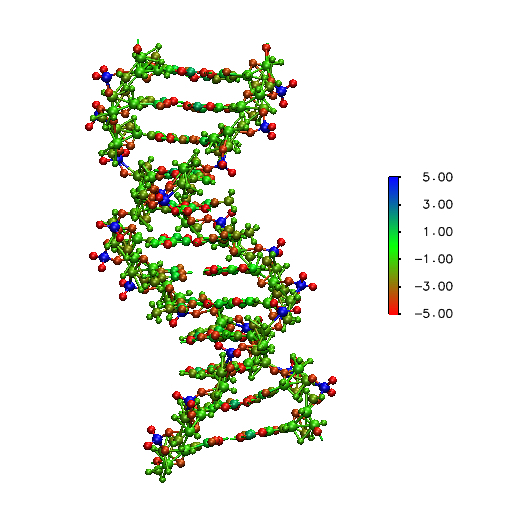
\includegraphics[scale = .5]{1bna_charge}
	\caption{Structure of a DNA (\textit{1bna}) constructed from its {\it .pqr} file showing atomic charges in color for each atoms.} 
\end{figure}

 In a \textit{.pdb} file for a particular protein, ATOM record type (the rows starting with the word "ATOM") contains the information about each atom as shown in Table \ref{tab:PDB_format}. These raw information are not readily usable for our proposed solver. A Python script has been developed to follow the following steps,
 
%\begin{enumerate}
\begin{itemize}
 	\item Reading \textit{.pdb} file RCSB website: The Python module \textit{"requests"} has been used to read and parse protein data from the web from the web address 'https://files.rcsb.org/view/' to write a local \textit{.pdb} file. 
	\item Converting  local \textit{.pdb} file to \textit{.pqr} file: The PDB2PQR software \cite{PDB2PQR} has been used to calculate the {\it .pqr} file. These \textit{.pqr} files contain ATOM record types similar to \textit{.pdb} files where the occupancy columns (55-60) and Temperature factor columns (61-66) have been replaced by the charge and radius.     
	%\item Parsing ATOM record types to collect $X,Y$ and $Z$ cor
 \end{itemize}
% \end{enumerate}

Finally in \textit{.pqr} files we have the $X,Y$ and $Z$ co-ordinate, the charge of the atomic center and the radius for each individual atom.   

\chapter{CLEANING THE OLD ADIMSMS CODING PACKAGE FOR THE NEW SIMULATIONS}
\label{chap: cleaning}
For our simulations we started with the ADIMSMS solver (a coding package) developed by Professor Shan Zhao, Dr. Weihua Geng form Southern Methodists University and Lieghton Wilson a former Masters Student at the Department of Mathematics at UA for their earlier work in \cite{Geng2013_Fully, Wilson2016}. F  
% --------------------------- Chapter 2 ----------------------------------------
\chapter{POISSON-BOLTZMANN EQUATION (PBE)}
\label{chap: PBE}
We are considering the Poisson-Boltzmann Equation (PBE) as the governing equation for a solute macro molecule immersed in an aqueous solvent environment illustrated in Fig 1. Our computational domain $\Omega \in \mathbb{R}^3$ is separated into two regions $\Omega^-$ and $\Omega^+$ by the molecular surface $\Gamma$, which is an arbitrarily shaped dielectric interface. Here $\Omega^-$ is the molecule domain with dielectric constant $\epsilon^-$ and $\Omega^+$ is the solvent domain with dielectric constant $\epsilon^+$. The cubic shape boundary of $\Omega= \Omega^-\cup \Omega^+ $ is denoted by $\delta \Omega$. The charges inside $\Omega^-$ has been distributed as the partial charges to assign to the nearest grid points to the center of each atom inside the molecule. The charges outside in $\Omega^+$ are mobile ions which are described by the Boltzmann distribution. Then the electrostatic interaction of this solute-solvent system for $\textbf{r} \in \mathbb{R}^3$ is governed by the nonlinear Poisson-Boltzmann Equation (PBE) as, 
\begin{equation}
			-\nabla.(\epsilon(\textbf{r})\nabla \phi(\textbf{r}))+\bar\kappa^2(\textbf{r}) \sinh (\phi(\textbf{r}))=\rho(\textbf{r})\label{pbe} %\\
					%\left[\phi \right]_\Gamma = 0 \textnormal{ and } \left[\epsilon\phi_n\right]_\Gamma = 0 
\end{equation}
with the boundary condition,
\begin{equation}
	\phi_b (\textbf{r}) = \frac{e_c^2}{k_B T} \sum_{i=1}^{N_c} \frac{q_i e^{-|\textbf{r}-\textbf{r}_i | \sqrt{\frac{\bar\kappa^2}{\epsilon^+}} }}{\epsilon^{+}|\textbf{r}-\textbf{r}_i|} \label{bd_cond}
\end{equation}
where the singular source $\rho(\textbf{r})$ term is defined as,
\begin{equation}
	\rho(\textbf{r})= 4\pi \frac{e_c^2}{k_B T}\sum_{i=1}^{N_c} q_i \delta(\textbf{r}-\textbf{r}_i) \label{rho}
\end{equation}
There are two conditions on $\Gamma$ needed to be satisfied from the dielectric theory for the potential $\phi$ and flux density $\epsilon \phi_\textbf{n} $, 
\begin{equation}
\left[\phi \right]_\Gamma = 0 \textnormal{ and } \left[\epsilon\phi_n\right]_\Gamma = 0 \label{ju_cond}
\end{equation}
Here $\textbf{n}=(n_x,n_y,n_z)$ is the outer normal direction on the interface $\Gamma$ and $\phi_\textbf{n}= \frac{\partial \phi}{\partial\textbf{n}} $ is the directional derivative in \textbf{n}. The notation $[f]_\Gamma = f^+-f^-$ represent the difference of the functional value across the interface $\Gamma$. 

The dielectric constant $\epsilon$ is piecewise such that, $\epsilon(\textbf{r})=\epsilon^-$ for $\textbf{r} \in \Omega^-$ and $\epsilon(\textbf{r})=\epsilon^+$ for $\textbf{r} \in \Omega^+$. Here $N_c$ is the total number of atoms in the solute molecule, $k_B$ is the Boltzmann constant, $e_c$ is the fundamental charge and $q_i$, in the same unit as $e_c$ is the partial charge on the \textit{i}th atom of the solute molecule located at position $\textbf{r}_j$. The Debey-Huckel parameter $\bar\kappa^2 =\Big(\frac{2N_A e_c^2}{100 k_b T}\Big)I_s =  8.486902807$\AA$^{-2} I_s$ \cite{Holst:1993} for $\textbf{r} \in \Omega^-$ and $\bar\kappa=0$ for $\textbf{r} \in \Omega^+$. Here $N_A$ is Avogadro’s Number and $I_s$ is the molar ionic strength. The reader can refer to REF1 and REF2 for more details about definitions and units of these coefficients. 
\section{Two-component regularization for singular sources}
\label{2_comp_reg}
To avoid the difficulty due to the source term and the work for solving the Laplace equation we consider a two component regularization proposed by Cai, Wang and Zhao \cite{Cai2009}. For this regularization the electrostatic potential $\phi$ has been considered as the addition of the coulmb component $\phi_c$ and the reaction field component $\phi_{RF}$ as $\phi= \phi_c +\phi_{RF}$. Here $\phi_c$ satisfies the following Poission's equation, 
\begin{equation}
	\begin{cases}
		-\epsilon^- \Delta\phi_C(r) = \rho(r) \text{   in   }\mathbb{R}^3 \label{rho_eq} \\
		\text{      }\phi_C(r)= 0. \text{   as  } |r| \rightarrow \infty
	\end{cases}
\end{equation}
which gives us the analytical solution as the Green's function $G$ for $\phi_C$ as,
\begin{equation}
	G(r) = \frac{e_c^2}{k_B T } \sum_{i=1}^{N_c} \frac{q_i }{\epsilon^{-}|r-r_i|} \label{Green} %\text{ where } C = \frac{e_c^2}{k_B T }
\end{equation}
	
%	Now the non-linear PBE from (\ref{pbe}) can be rewritten as,
%	
%	  \begin{eqnarray}
%				-\nabla.(\epsilon\nabla (\phi_C(\textbf{r})))-\nabla.(\epsilon\nabla (\phi_{RF}(\textbf{r})))+\bar\kappa^2(\textbf{r}) \sinh (\phi_C(\textbf{r})+\phi_{RF}(\textbf{r}))&=&\rho(\textbf{r}), \text{ in } \Omega \label{pbe_reg} %\\
%						%\left[\phi \right]_\Gamma = 0 \textnormal{ and } \left[\epsilon\phi_n\right]_\Gamma = 0 
%	\end{eqnarray}
%	
%	The reaction field components can be physically interpreted as the electrostatic field generated by the charges induced by changes of dielectric constant of the  solvent around the solute from $\epsilon^-$ to $\epsilon^+$ \cite{Cai2009}. Now substituting (\ref{rho}) into (\ref{pbe_reg}) we have,
%	\begin{eqnarray}
%	-\nabla(\epsilon^+ \phi_{RF}(\textbf{r})) +\bar\kappa^2 \sinh(\phi_C(\textbf{r})+\phi_{RF}(\textbf{r}))&=& 0 \text{ in } \Omega^- \cup \Omega^+	
%	\end{eqnarray}
%	More explicitly $\phi_{RF}$ satisfies the following elliptic interface problem \cite{Chen2007}, 
%\begin{eqnarray}
%		-\nabla.(\epsilon^- \nabla  \phi_{RF}) &=& 0 \text{ in } \Omega^-\\  
%		-\nabla(\epsilon^+ \phi_{RF}) +\bar\kappa^2 \sinh(\phi_C+\phi_{RF})&=& 0 \text{ in } \Omega^+\\
%		\left[\phi_{RF}\right] &=& 0 \text{ on } \Gamma \\
%		\left[\epsilon\frac{\partial \phi_{RF}}{\partial n}\right]&=& (\epsilon^+-\epsilon^- ) \frac{\partial G}{\partial n} \text{ on } \Gamma\\
%		\phi_{RF}&=& \phi_b-G \text{ on } \partial \Omega \label{rf_sys}
%	\end{eqnarray} 
%	
%So now there is no singular term on the right hand side but we still have several numerical difficulties. In \cite{Holst2010} its been reported that $\phi_C$ and $\phi_{RF}$ have different signs and their magnitude is much larger than that of $\phi$. Here  a relatively small error in $\phi_{RF}$ will produce a relatively larger error in $\phi$ given that the $phi_C$ is analytically calculated. Sometimes this amplifying factor can be as large as $(\epsilon^+/\epsilon^- - 1 )$ \cite{Holst2010}. In our case this factor is about $79$ by taking $\epsilon^+=80$ and $\epsilon^-=1$. Another problem is, the calculation of $\phi_C$ is necessary for all N grid points in $\Omega^+$ at a computational cost $O(N^2)$ which is very expensive for large $N$. 
%
Then Luo and his collaborators \cite{Cai2009} proposed to solve for the original solution $\phi$ in $\Omega^+$ instead of the reaction component $\phi_{RF}$. Now to make the required adjustments to fit this regularization approach \cite{Cai2009} with finite difference and finite element method Zhao and Geng \cite{Geng2017a} proposed a new elliptic problem with discontinuous function flux jumps for the two-component regularization. In particular they defined the regularized potential as,  
	
\begin{eqnarray}
	\tilde{ \phi} &=& \begin{cases}
	\phi_{RF} \text{ in } \Omega^-\\
	\phi_C + \phi_{RF} \text{ in } \Omega^+\\
	\end{cases}
\end{eqnarray}
 
The jump conditions for $\tilde\phi $ were derived from $\phi$ and the definition $\phi=\phi_C+\phi_{RF}$ as,

\begin{eqnarray}
\phi^+=\phi^-_{RF}+\phi^-_C,\text{  and  } \epsilon^+ \frac{\partial \phi^+}{\partial n}=\epsilon^- \frac{\partial \phi^-_{RF}}{\partial n}+\epsilon^- \frac{\partial \phi^-_C}{\partial n} \text{ on } \Gamma
\end{eqnarray}

Thus, the regularized PB equation of $\tilde \phi$ with corresponding interface and boundary conditions are given as. 
\begin{eqnarray}
	-\nabla.(\epsilon^- \nabla \tilde{ \phi}) &=& 0 \text{ in } \Omega^-\\ \label{phitilde1}
	-\nabla.(\epsilon^+ \nabla \tilde{ \phi}) +\bar\kappa^2 \sinh(\tilde{ \phi})&=& 0 \text{ in } \Omega^+\\\label{phitilde2}
	\left[\tilde{ \phi}\right] &=& G \text{ on } \Gamma \\ \label{phitilde3}
	\left[\epsilon\frac{\partial \tilde{ \phi}}{\partial n}\right]&=& \epsilon^-  \frac{\partial G}{\partial n} \text{ on } \Gamma\\\label{phitilde4}
	\tilde{\phi} &=& \phi_b \text{ on } \partial \Omega \label{phitilde5}
\end{eqnarray}	
	


Now from (\ref{phitilde1}) and (\ref{phitilde5}) we can summarize that, 

\begin{eqnarray}
	-\nabla . (\epsilon \nabla \tilde{ \phi}) +\bar\kappa^2 \sinh(\tilde{ \phi})&=& 0 \text{ in } \Omega^-\cup\Omega^+\label{RPB}
\end{eqnarray}
	 
where $\tilde \phi$	 satisfies the PB equation without the source term. Then Zhao and Geng \cite{Geng2017a} proposed to numerically solve the regularized PB interface problem (RPB) given in (\ref{phitilde1})-(\ref{phitilde5}) and to finally recover the original solution as $\phi= \tilde\phi $ in $\Omega^+$ and $\phi = \tilde \phi + G $ in $\Omega^-$, Where the Green's function $G$ is analytically given.
\section{Solvation energy from Electrostatic potential}

The solvation energy can be defined as the energy released when the solute in free space is dissolved in solvent and it can be expressed in terms of the electrostatic free energy $\Delta G_{\rm ele}$ and the coulomb energy $E_{\rm cou}$ as 

\begin{eqnarray}
	\Delta G_{\rm ele}&=& E_{\rm cou}+ E_{\rm sol}\label{eq_Gele}\\
	E_{\rm cou} &=& \sum_{i=1}^{N_c}\sum_{j=1}^{N_c}\frac{q_iq_j}{\epsilon^-d_{i,j}}, i\neq j\label{eq_Ecou}
\end{eqnarray}
where $q_i$ and $q_j$ are the charges at the center of the atoms and $d_{i,j}$'s are the distance between the $i$-th and $j$-the atom. 
  
Then Sharp and Honig in \cite{Sharp_Honig}  described the calculation electrostatic free energy by, 
\begin{equation}
\Delta G_{\rm ele}=\int_{\mathbb{R}^3}\left(\phi\rho+\Delta\Pi-\frac{1}{2}\epsilon|{\bf E}|^2\right)d{\bf r}
\end{equation}

where $\phi$ is the electrostatic potential, $\rho$ is the fixed charge density represented as a smeared surface charge or as a collection of point charges, $\Delta\Pi$ is  the excess osmotic pressure of the mobile ion cloud, and $\frac{1}{2}\epsilon|{\bf E}|^2$ is the electrostatic stress.

Now for the simplification of the numerical validations of our proposed schemes in the next chapter we omitted the energy components related to the mobile ion pressure and the electrostatic stress to report the solvation energy $E_{\rm sol}$ as,  

\begin{eqnarray}
	E_{\rm sol}=\Delta G_{\rm ele}-E_{\rm cou}\approx\sum\limits_{i=1}^{N_c}q_i\phi_{RF} ({\bf r}_i)\label{eq_solvation}
\end{eqnarray}

Here the contribution of the mobile ion pressure and the electrostatic stress to the whole calculation is really small and computationally more challenging. The readers can refer to \cite{GENG_WEI2011,Gilson,Sharp_Honig} for more details.				


\section{Pseudo-transient continuation approach for the PBE}

As the pseudo-transient continuation approach, an indirect method discussed in \cite{zhao_pseudo-time-coupled_2011} \cite{Sayyed-Ahmad2004} \cite{shestakov_solution_2002} introduced a pseudo-time derivative to solve the PB equation as,  

\begin{eqnarray}
	 	\frac{\partial u}{\partial t} &=& \nabla.(\epsilon \nabla u)-\bar\kappa^2 \sinh(u) \text{ in } \Omega^- \cup \Omega^+ \label{tdrpb} \\
	 	  \left[u\right]&=& G,\text{ and } \left[\epsilon\frac{\partial u}{\partial n}\right]= \epsilon^-  \frac{\partial G}{\partial n} \text{ on } \Gamma\\ \label{jump}
	 	  u&=&\phi_b \text{ on } \partial \Omega
	\end{eqnarray}

Here the time independent regularized PB equation in (\ref{RPB}) has been converted in to a time dependent regularized PB (TDRPB) in (\ref{tdrpb}). Our goal is to first specify the initial condition, which could be the electrostatic potential solved from a linearized PB \cite{zhao_pseudo-time-coupled_2011} equation or trivially $u = 0$ and then numerically integrate (\ref{tdrpb}) for a sufficiently long period to get the steady state solution as the solution of the original regularized PB (\ref{RPB}). Here the sign on the right hand side of eq. (\ref{tdrpb}) has been considered as the reverse of the eq.(\ref{RPB}) to ensure the numerical stability. 

But, there are difficulties in the numerical integration of the TDRPB equation (\ref{tdrpb}) because of the requirement of long time integration, when explicit time stepping methods are usually not efficient \cite{Sayyed-Ahmad2004},\cite{shestakov_solution_2002},\cite{zhao_pseudo-time-coupled_2011}, \cite{zhao_operator_2014}. Hence we are employing a semi-implicit time splitting method \cite{Sayyed-Ahmad2004},\cite{shestakov_solution_2002} which have been commonly used to solve the TDPB in the literature. 


% --------------------------- Chapter 3 ----------------------------------------
\chapter{OPERATOR SPLITTING SCHEMES}
\label{chap:opt_split}
\section{Two-component regularization for singular sources}
\label{2_comp_reg}
To avoid the difficulty due to the PBE for the vacuum case Cai, Wang and Zhao \cite{Cai2009} proposed a two component regularization. For this regularization the electrostatic potential $\phi$ is expressed as the sum of the coulomb component $\phi_c$ and the reaction field component $\phi_{RF}$.
% as $\phi= \phi_c +\phi_{RF}$. 
Here $\phi_c$ satisfies the following Poisson's equation, 
\begin{equation}
	\begin{cases}
		-\epsilon^- \Delta\phi_C({\bf r}) = \rho({\bf r}) \text{   in   }\mathbb{R}^3 \label{rho_eq}, \\
		\text{      }\phi_C({\bf r})= 0. \text{   as  } |{\bf r}| \rightarrow \infty.
	\end{cases}
\end{equation}\label{eq:cl_comp}
which has the analytical solution as the Green's function $G$ for $\phi_C$ as,
\begin{equation}
	G({\bf r}) = \frac{e_c^2}{k_B T } \sum_{i=1}^{N_c} \frac{q_i }{\epsilon^{-}|{\bf r}-{\bf r}_i|}. \label{eq:green} %\text{ where } C = \frac{e_c^2}{k_B T }
\end{equation}
Now the PBE from equation (\ref{pbe}) can be rewritten as,
\begin{equation}
		-\nabla.(\epsilon\nabla (\phi_C(\textbf{r})))-\nabla.(\epsilon\nabla (\phi_{RF}(\textbf{r})))+\bar\kappa^2(\textbf{r}) \sinh (\phi_C(\textbf{r})+\phi_{RF}(\textbf{r}))=\rho(\textbf{r}). \label{pbe_reg} %\\
				%\left[\phi \right]_\Gamma = 0 \textnormal{ and } \left[\epsilon\phi_n\right]_\Gamma = 0 
\end{equation}
The reaction field component $\phi_{RF}$ can be physically interpreted as the electrostatic field generated by the charges induced by replacing the solvent around the solute molecule. It changes the dielectric constant in $\Omega^+$ form $\epsilon^+$ to $\epsilon^-$ \cite{Cai2009}. Now substituting (\ref{eq:cl_comp}) into (\ref{pbe_reg}) we have,
\begin{eqnarray}
-\nabla(\epsilon^+ \phi_{RF}(\textbf{r})) +\bar\kappa^2 \sinh(\phi_C(\textbf{r})+\phi_{RF}(\textbf{r}))&=& 0 \text{ in } \Omega^- \cup \Omega^+.	
\end{eqnarray}
More explicitly, $\phi_{RF}$ satisfies the following elliptic interface problem as described in \cite{Chen2007}: 
\begin{eqnarray}
		-\nabla.(\epsilon^- \nabla  \phi_{RF}) &=& 0 \text{ in } \Omega^-,\\  
		-\nabla(\epsilon^+ \phi_{RF}) +\bar\kappa^2 \sinh(\phi_C+\phi_{RF})&=& 0 \text{ in } \Omega^+,\\
		\left[\phi_{RF}\right] &=& 0 \text{ on } \Gamma, \\
		\left[\epsilon\frac{\partial \phi_{RF}}{\partial n}\right]&=& (\epsilon^+-\epsilon^- ) \frac{\partial G}{\partial n} \text{ on } \Gamma,\\
		\phi_{RF}&=& \phi_b-G \text{ on } \partial \Omega ,\label{rf_sys}
\end{eqnarray} 
Now there is no singular term on the right hand side but we still have several numerical difficulties left to address. It is known that $\phi_C$ and $\phi_{RF}$ have different signs and their magnitude is much larger than $\phi$ \cite{Holst2010}. It can be shown \cite{Holst2010} using the benchmark problem called Born Ion that, a relatively small error in $\phi_{RF}$ will produce a relatively larger error in $\phi$ given that the $\phi_C$ is analytically calculated. Sometimes this amplifying factor \cite{Holst2010} can be as large as $(\epsilon^+/\epsilon^- - 1 )$. In our case this factor is about $79$ by taking $\epsilon^+=80$ and $\epsilon^-=1$. Another problem is the calculation of $\phi_C$ is necessary at all N grid points in $\Omega^+$ at a computational cost $O(N^2)$ which is very expensive for large $N$. 

These difficulties motivated us to consider a newer version of the two component regularization proposed by Luo et al. in \cite{Cai2009}. They proposed to solve for the whole original solution $\phi$ in $\Omega^+$ instead of the reaction component $\phi_{RF}$ only. Then to make the required adjustments to fit this regularization approach with finite difference and finite element methods, Zhao and Geng \cite{Geng2017a} proposed a new interface problem with discontinuous flux jumps for the regularized potential $\tilde \phi$. In particular they defined it as 
\begin{eqnarray}
	\tilde{ \phi} &=& \begin{cases}
	\phi_{RF} \text{ in } \Omega^-\\
	\phi_C + \phi_{RF} \text{ in } \Omega^+\\
	\end{cases}.
\end{eqnarray}
 The jump conditions for $\tilde\phi $ were derived from the definition $\phi=\phi_C+\phi_{RF}$ as
\begin{eqnarray}
\phi^+=\phi^-_{RF}+\phi^-_C \text{  and  } \epsilon^+ \frac{\partial \phi^+}{\partial n}=\epsilon^- \frac{\partial \phi^-_{RF}}{\partial n}+\epsilon^- \frac{\partial \phi^-_C}{\partial n} \text{ on } \Gamma.
\end{eqnarray}
Hence, the regularized PBE (RPBE) with the corresponding interface and the boundary conditions takes the following form: 
\begin{eqnarray}
	-\nabla.(\epsilon^- \nabla \tilde{ \phi}) &=& 0 \text{ in } \Omega^-,\label{phitilde1}\\ 
	-\nabla.(\epsilon^+ \nabla \tilde{ \phi}) +\bar\kappa^2 \sinh(\tilde{ \phi})&=& 0 \text{ in } \Omega^+,\label{phitilde2}\\
	\left[\tilde{ \phi}\right] &=& G \text{ on } \Gamma, \label{phitilde3}\\ 
	\left[\epsilon\frac{\partial \tilde{ \phi}}{\partial n}\right]&=& \epsilon^-  \frac{\partial G}{\partial n} \text{ on } \Gamma,\label{phitilde4}\\
	\tilde{\phi} &=& \phi_b \text{ on } \partial \Omega. \label{phitilde5}
\end{eqnarray}	
Now we can summarize equation (\ref{phitilde1}) and equation (\ref{phitilde2}) as
\begin{equation}
	-\nabla . (\epsilon \nabla \tilde{ \phi}) +\bar\kappa^2 \sinh(\tilde{ \phi})=0 \text{ in } \Omega^-\cup\Omega^+.\label{eq:RPBE}
\end{equation}
 Zhao and Geng \cite{Geng2017a} proposed to numerically solve the regularized PB interface problem (RPBE) given in (\ref{phitilde1})-(\ref{phitilde5}) for $\tilde \phi$ and recovered the original solution as $\phi= \tilde\phi $ in $\Omega^+$ and $\phi = \tilde \phi + G $ in $\Omega^-$. Here the Green's function $G$ can be calculated analytically from  (\ref{eq:green}). We note that in  jump conditions (\ref{phitilde3}) and (\ref{phitilde4}) both the solution and its flux are discontinuous. 
%%%%%%%%%%%%%%%%%%%%%%%%%%%%%%%%%%%%%%%%%%%%%%%%%%%%%%%%%%%%%%%%%%%%%%%%%%%%%
\section{Pseudo-transient approach for the TRPBE}

As the ADI method in Section \ref{sec:adi-method}, a pseudo-time derivative has been introduced in the RPBE to solve the PBE as,  

%\begin{eqnarray}
%	 	\frac{\partial u}{\partial t} &=& \nabla.(\epsilon \nabla u)-\bar\kappa^2 \sinh(u) \text{ in } \Omega^- \cup \Omega^+ \label{eq:TRPBE} \\
%	 	  \left[u\right]&=& G,\text{ and } \left[\epsilon\frac{\partial u}{\partial n}\right]= \epsilon^-  \frac{\partial G}{\partial n} \text{ on } \Gamma\\ \label{jump}
%	 	  u&=&\phi_b \text{ on } \partial \Omega
%\end{eqnarray}
\begin{eqnarray}
	 	\frac{\partial \tilde\phi(\textbf{r},t)}{\partial t} &=& \nabla.(\epsilon({\bf r}) \nabla \tilde\phi(\textbf{r},t))-\bar\kappa^2({\bf r}) \sinh(\tilde\phi(\textbf{r},t)) \text{ in } \Omega^- \cup \Omega^+ \label{eq:TRPBE}. %\\
	 	  %\left[u\right]&=& G,\text{ and } \left[\epsilon\frac{\partial u}{\partial n}\right]= \epsilon^-  \frac{\partial G}{\partial n} \text{ on } \Gamma\\ \label{jump}
	 	%  u&=&\phi_b \text{ on } \partial \Omega
\end{eqnarray}
Here the time independent RPBE in (\ref{eq:RPBE}) has been converted into a time dependent regularized PBE (TRPBE) in (\ref{eq:TRPBE}). Unlike TPBE in (\ref{eq:tpbe}), TRPBE does not have any singular term $\rho({\bf r})$.   

As the initial condition, we used the electrostatic potential solved from a linearized PBE \cite{Zhao2011} or trivially $\tilde \phi= 0$. Then we numerically integrate (\ref{eq:TRPBE}) for a sufficiently long period to get the steady state solution as the solution of the original regularized PBE (\ref{eq:RPBE}). Here the sign on the right hand side of equation (\ref{eq:TRPBE}) has been considered as the reverse of the equation(\ref{eq:RPBE}) to ensure the numerical stability. 

However, there are still some challenges left for the numerical integration of the TRPBE (\ref{eq:TRPBE}) because of the requirement of long time integration, when explicit time stepping methods are usually not efficient \cite{Sayyed-Ahmad2004,Shestakov2002,Zhao2011,zhao_operator_2014}. Hence we employ a semi-implicit time splitting method \cite{Sayyed-Ahmad2004,Shestakov2002}, which have been commonly used to solve the TPBE (\ref{eq:tpbe}) in the literature. 

Let us consider a uniform mesh with a grid spacing $h$ in all $x,y$ and $z$ directions having $N_x,N_y$ and $N_z$ as the number of the grid points in each direction. We assume the vector ${{\bf u}^n = \tilde \phi^n_{ijk}}$ for $i=1,...., N_x,j=1,...,$ and $N_y,k=1,...N_z$ denote all the nodal values of $\tilde \phi$ at the time level $t_n$. We use two stages to update ${\bf u^n}=\tilde \phi^n$ at time level $t_n$ to ${\bf u^{n+1}}=\tilde \phi^{n+1}$ at time level $t_{n+1}=t_n+ \Delta t $. In these two stages at each time step we develop several types of operator splitting schemes for updating ${\bf u}^n$. 
  %%%%%%%%%%%%%%%%%%%%%%%%%%%%%%%%%%%%%%%%%%%%%%%%%%%%%%%%%%%%%%%%%%%%%%%%%%%%%
\section{Operator Splitting for the GFM-ADI method}
%\section{ADI method with Implicit-Euler method (GFM-ADI)}
\label{sec:GFM-ADI}

In this scheme at the first stage, TRPBE in  (\ref{eq:TRPBE}) will be solved by a first order time splitting into the two following equations similar to the ADI method discussed in Section (\ref{sec:adi-method}): 
\begin{eqnarray}
  \frac{\partial w}{\partial t}&=& -\bar\kappa^2 \sinh(w) \text{ with } {\bf w}^n={\bf u}^n\text{ and } t \in \left[t_n,t_{n+1}\right],\label{eq:non_linear_ADI}\\
 \frac{\partial v}{\partial t}&=&  \nabla . (\epsilon\nabla v) \text{ with } {\bf v}^n={\bf w}^{n+1}\text{ and } t \in \left[t_n,t_{n+1}\right].	 \label{eq:diffusion_ADI}
\end{eqnarray}  
For the first equation, (\ref{eq:non_linear_ADI}), we will use the analytical solution ${\bf w}^{n+1}=F({\bf w}^n,\Delta t)$ defined in (\ref{eq:anal_sol}). Then for the temporal discretization of the equation (\ref{eq:diffusion_ADI}) we use the Backward-Euler integration in time to get 
\begin{equation}
	v_{i,j,k}^{n+1} =v_{i,j,k}^{n}+\Delta t \left(\delta_x^2+\delta_y^2+\delta_z^2\right)v_{i,j,k}^{n+1}. \label{eq:imp-eu}
\end{equation}	
We cannot use the definition of $\Delta_x^2,\Delta_y^2$ and $\Delta_z^2$ in (\ref {eq:dif_opx_adi1}) for $\delta_x^2,\delta_y^2$ and $\delta_z^2$, since both the potential function $\tilde \phi$ and its flux are discontinuous on the interface $\Gamma$ as in equations (\ref{phitilde3}) and (\ref{phitilde4}). So we define $\delta_x^2,\delta_y^2$ and $\delta_z^2$ as a central finite difference operators in (\ref{dif_opz}) in the $x,y$ and $z$ directions, respectively with 
\begin{equation}
	\epsilon_{i,j,k}= \displaystyle\begin{cases}
	\epsilon^- \text{ if } x_{i,j,k}\in\Omega^- \cup \Gamma \\
	\epsilon^+ \text{ if } x_{i,j,k}\in\Omega^+
	\end{cases},
\end{equation}
as
 \begin{eqnarray}
 \begin{aligned}
	\delta_x^2\left(v_{i,j,k}^n\right)&= \frac{\epsilon_{i,j,k}}{h^2} \left(v_{i-1,j,k}^n-2v_{i,j,k}^n+v_{i+1,j,k}^n\right), \\ \label{dif_opx}
	\delta_y^2\left(v_{i,j,k}^n\right)&= \frac{\epsilon_{i,j,k}}{h^2} \left(v_{i,j-1,k}^n-2v_{i,j,k}^n+v_{i,j+1,k}^n\right),\\ %\label{dif_opy}
	\delta_z^2\left(v_{i,j,k}^n\right)&= \frac{\epsilon_{i,j,k}}{h^2} \left(v_{i,j,k-1}^n-2v_{i,j,k}^n+v_{i,j,k+1}^n\right). \label{dif_opz}
\end{aligned}
\end{eqnarray}
Even though these three point stencils for $\delta_x^2,\delta_y^2$ and $\delta_z^2$ give a huge advantage for the regular grid points, it posses a difficulty for the points adjacent to the interface. We will discuss more about this difficulty later in Chapter \ref{chap:new_GFM}.
  
Now for the second stage of the operator splitting, a first order Douglas-Rachford type ADI scheme is used to decompose the diffusion equation, (\ref{eq:imp-eu}), in $x,y$ and $z$ directions as  
\begin{eqnarray}
%\begin{aligned}
		\left(1- \Delta t \delta_x^2\right)v_{i,j,k}^{*}&=&\left[1+ \Delta t \left(\delta_y^2+\delta_z^2 \right)\right]v_{i,j,k}^{n},\label{GFM-ADI}\\
		\left(1-\Delta t \delta_y^2\right)v_{i,j,k}^{**}&=&v_{i,j,k}^{*}- \Delta t \delta_y^2\left(v_{i,j,k}^{n}\right),\label{GFM-ADI2}\\
		\left(1- \Delta t \delta_z^2\right)v_{i,j,k}^{n+1}&=&v_{i,j,k}^{**}- \Delta t \delta_z^2\left(v_{i,j,k}^{n}\right).\label{GFM-ADI3}
%\end{aligned}		\label{1dadi}
\end{eqnarray} 
where $v^*$ and $v^{**}$ are two intermediate values to create three tridiagonal one-dimensional systems. Here, the three dimensional linear algebraic system in equation (\ref{eq:imp-eu}) has been decomposed into several one dimensional linear algebraic systems in (\ref{GFM-ADI}), (\ref{GFM-ADI2}) and (\ref{GFM-ADI3}). The finite difference matrix for each one these linear equations has a tridiagonal structure. These three tridiagonal systems are much more efficient to solve because of the tridiagonal symmetry than one non-structured system (\ref{eq:imp-eu}). Then by eliminating $v^*_{i,j,k}$ and $v^{**}_{i,j,k}$ and solving for $v^{n+1}_{i,j,k}$ in (\ref{eq:imp-eu}) we get,
\begin{eqnarray}
\begin{aligned}
	v^{n+1}_{i,j,k}&=v^n_{i,j,k}+ \Delta t \left(\delta_x^2+\delta_y^2+\delta_z^2\right) v^{n+1}_{i,j,k} -\Delta t^2 \left(\delta_x^2\delta_y^2+\delta_x^2\delta_y^2+\delta_z^2\delta_y^2\right)(v^{n+1}_{i,j,k}-v^{n}_{i,j,k})\\
	&+ \Delta t^3 \delta_x^2\delta_y^2\delta_z^2(v^{n+1}_{i,j,k}-v^{n}_{i,j,k}). \label{adi_tailor}
	\end{aligned}
\end{eqnarray}
Hence the Douglas-Rachford scheme (\ref{eq:imp-eu}) is a higher order perturbation of the Implicit-Euler method. Since both (\ref{eq:non_linear_ADI}) and (\ref{eq:diffusion_ADI}) are first order in time this proposed GFM-ADI method is of first order accuracy in time. For the boundary conditions we use the same Dirichlet boundary boundary values from equation (\ref{bd_cond}) for $v$, $v^*$ and  $v^{**}$ for $u$. The entire time integration here is fully implicit. 


%%%%%%%%%%%%%%%%%%%%%%%%%%%%%%%%%%%%%%%%%%%%%%%%%%%%%%%%%%%%%%%%%%%%%%%%%%%%%
\section{Operator Splitting for the GFM-LODCN method}
%\section{LOD with Crank-Nicolson method(GFM-LODCN)}\label{GFM-LODCN}
\label{sec:GFM-LODCN}
In this operator splitting scheme at each time step from $t_n$ to $t_{n+1}$, the TRPBE (\ref{eq:TRPBE}) is splitted into the following three equations by a second order time splitting method \cite{Yu2005}:
\begin{eqnarray}
  \frac{\partial w}{\partial t}&=& -\frac{1}{2}\bar\kappa^2 \sinh(w) \text{ with } {\bf w}^n={\bf u}^n\text{ and } t \in \left[t_n,t_{n+1}\right],\label{non_linear1_LOD-CN}\\
 \frac{\partial v}{\partial t}&=&  \nabla . (\epsilon\nabla v) \text{    with } {\bf v}^n={\bf w}^{n+1}\text{ and } t \in \left[t_n,t_{n+1}\right],	 \label{diffusion_LOD-CN}\\
 \frac{\partial \tilde{w}}{\partial t}&=& -\frac{1}{2}\bar\kappa^2 \sinh( \tilde{w}) \text{ with } \tilde{\bf w}^n={\bf v}^{n+1}\text{ and } t \in \left[t_n,t_{n+1}\right].\label{non_linear2_LOD-CN}
\end{eqnarray}
We then have ${\bf u}^{n+1}=\tilde{\bf w}^{n+1}$. Similar to the GFM-ADI method in Section (\ref{sec:GFM-ADI}), at the first stage we use an analytical integration for the nonlinear equations, (\ref{non_linear1_LOD-CN}) and (\ref{non_linear2_LOD-CN}). Symbolically, we have ${\bf w}^{n+1}=F({\bf w}^n,\frac{\Delta t}{2})$ and $\tilde{\bf w}^{n+1}=F(\tilde{\bf w}^n,\frac{\Delta t}{2})$, where $F$ is defined in equation (\ref{eq:anal_sol}).

Then for the second stage, we propose another multiplicative operator splitting scheme, called the Locally One Dimensional (LOD) scheme to solve the diffusion equation (\ref{diffusion_LOD-CN}). These types of fractional step methods were first developed by Russian mathematicians \cite{Yakonov_1963,Yanenko_1963,Yanenko_1967}. The discretization of equation (\ref{diffusion_LOD-CN}) using Crank-Nicolson integration in time and central differencing in space results in, 
\begin{eqnarray}
	\left(1-\frac{\Delta t}{2}(\delta^2_x+\delta^2_y+\delta^2_z)\right)v_{i,j,k}^{n+1}=\left(1+\frac{\Delta t}{2}(\delta^2_x+\delta^2_y+\delta^2_z)\right)v_{i,j,k}^n,
\end{eqnarray}
which can be decomposed into $x,y$ and $z$ directions to give the LOD scheme for (\ref{diffusion_LOD-CN}) as
\begin{eqnarray}
	\left(1-\frac{\Delta t}{2}\delta_x^2\right)v^*_{i,j,k}&=\left(1+\frac{\Delta t}{2}\delta_x^2\right)v^n_{i,j,k},\nonumber\\
	\left(1-\frac{\Delta t}{2}\delta_y^2\right)v^{**}_{i,j,k}&=\left(1+\frac{\Delta t}{2}\delta_y^2\right)v^*_{i,j,k},\nonumber\\
	\left(1-\frac{\Delta t}{2}\delta_z^2\right)v^{n+1}_{i,j,k}&=\left(1+\frac{\Delta t}{2}\delta_z^2\right)v^{**}_{i,j,k}.\nonumber\label{LODCN_eq}
\end{eqnarray}

Similar to the GFM-ADI method described in Section \ref{sec:GFM-ADI}, the tridiagonal systems in (\ref{LODCN_eq}) can be efficiently solved by the Thomas algorithm. 

%%%%%%%%%%%%%%%%%%%%%%%%%%%%%%%%%%%%%%%%%%%%%%%%%%%%%%%%%%%%%%%%%%%%%%%%%%%%%

\section{Operator Splitting for the GFM-LODIE method}
%\section{LOD with Implicit-Euler method (GFM-LODIE)}

For this method at each time step from $t_n$ to $t_{n+1}$, the TRPBE (\ref{eq:TRPBE}) is  solved in two stages similar to the GFM-ADI scheme described in Section \ref{sec:GFM-ADI}. 
The first stage is exactly the same to the GFM-ADI method. The first order time splitting is used for 
 TRPBE (\ref{eq:TRPBE}) to generate   equations (\ref{eq:non_linear_ADI}) and (\ref{eq:diffusion_ADI}). Equation (\ref{eq:non_linear_ADI}) is solved analytically by the function ${\bf w}^{n+1}=F({\bf w}^n,\Delta t)$ defined in equation (\ref{eq:anal_sol}).
 
 Then for the second stage, we apply the LOD scheme described in Section \ref{sec:GFM-LODCN} to decompose equation (\ref{eq:imp-eu}) in $x,y$ and $z$ directions:
 \begin{eqnarray}
		(1-\Delta t \delta_x^2)v^*_{i,j,k} &= v^n_{i,j,k},\nonumber\\
		(1-\Delta t \delta_y^2)v^{**}_{i,j,k} &= v^*_{i,j,k},\\
		(1-\Delta t \delta_z^2)v^{n+1}_{i,j,k} &= v^{**}_{i,j,k},\nonumber
\end{eqnarray}	
which are solved again individually by the Thomas Algorithm used in the previous sections. 

%%%%%%%%%%%%%%%%%%%%%%%%%%%%%%%%%%%%%%%%%%%%%%%%%%%%%%%%%%%%%%%%%%%%%%%%%%%%%%%%%%%%%
\section{Solvation energy from Electrostatic potential}

The solvation energy can be defined as the energy released when the solute from the free space is dissolved in the solvent and it can be expressed in terms of the electrostatic free energy $\Delta G_{\rm ele}$ and the coulomb energy $E_{\rm cou}$ as
\begin{equation}
	\Delta G_{\rm ele}= E_{\rm cou}+ E_{\rm sol},\label{eq_Gele}
\end{equation}
where
\begin{equation}	
	E_{\rm cou} = \sum_{i=1}^{N_c}\sum_{j=1}^{N_c}\frac{q_iq_j}{\epsilon^-d_{i,j}}, i\neq j,\label{eq_Ecou}
\end{equation}
and $q_i$ and $q_j$ are the charges at the center of the atoms, and $d_{i,j}$ is the distance between the $i$-th and $j$-th atom. 

Sharp and Honig \cite{Sharp_Honig} describe the calculation of the electrostatic free energy by using 
\begin{equation}
\Delta G_{\rm ele}=\int_{\mathbb{R}^3}\left(\phi\rho+\Delta\Pi-\frac{1}{2}\epsilon|{\bf E}|^2\right)d{\bf r},
\end{equation}
where $\phi$ is the electrostatic potential, $\rho$ is the fixed charge density represented as a smeared surface charge or as a collection of point charges, $\Delta\Pi$ is  the excess osmotic pressure of the mobile ion cloud, and $\frac{1}{2}\epsilon|{\bf E}|^2$ is the electrostatic stress.

For the simplification of the numerical validations of our proposed schemes in the Chapter \ref{chap:num_vald} we omitted the energy components related to the mobile ion pressure and the electrostatic stress to report the solvation energy $E_{\rm sol}$ as  
\begin{equation}
	E_{\rm sol}=\Delta G_{\rm ele}-E_{\rm cou}\approx\sum\limits_{i=1}^{N_c}q_i\phi_{RF} ({\bf r}_i).\label{eq:solvation}
\end{equation}
Here the contribution of the mobile ion pressure and the electrostatic stress to the whole calculation is really small and computationally more challenging. The readers can refer to \cite{GENG_WEI2011,Gilson,Sharp_Honig} for more details.	 

% --------------------------- Chapter 4 ----------------------------------------
\chapter{A NEW DERIVATION FOR GHOST FLUID METHOD}
\label{chap:new_GFM}
%on the points far away from the interface $\Gamma$ which are defined as regulars nodes.
At the points adjacent to the interface $\Gamma$, the central difference operators defined in (\ref{dif_opx})-(\ref{dif_opz}) are not used since these points are defined as irregular points where at-least one of its adjacent points is on the other side of the interface $\Gamma$. 
%On the irregular points at least one of the three point stencils for $\delta_x^2,\delta_y^2$ and $\delta_z^2$ is across the interface. 
Here the information about the function $v$ is not available for the point which is on the other side of the interface. A non-standard finite difference formula is necessary on the irregular points to discretize $\delta_x^2,\delta_y^2$ and $\delta_z^2$.  In this regard a modified version of the Ghost Fluid Method is proposed in this chapter using fictitious points (or ghost points) and the jump conditions given by (\ref{phitilde3}) and (\ref{phitilde4}).

\begin{figure}[!ht]
	\centering
	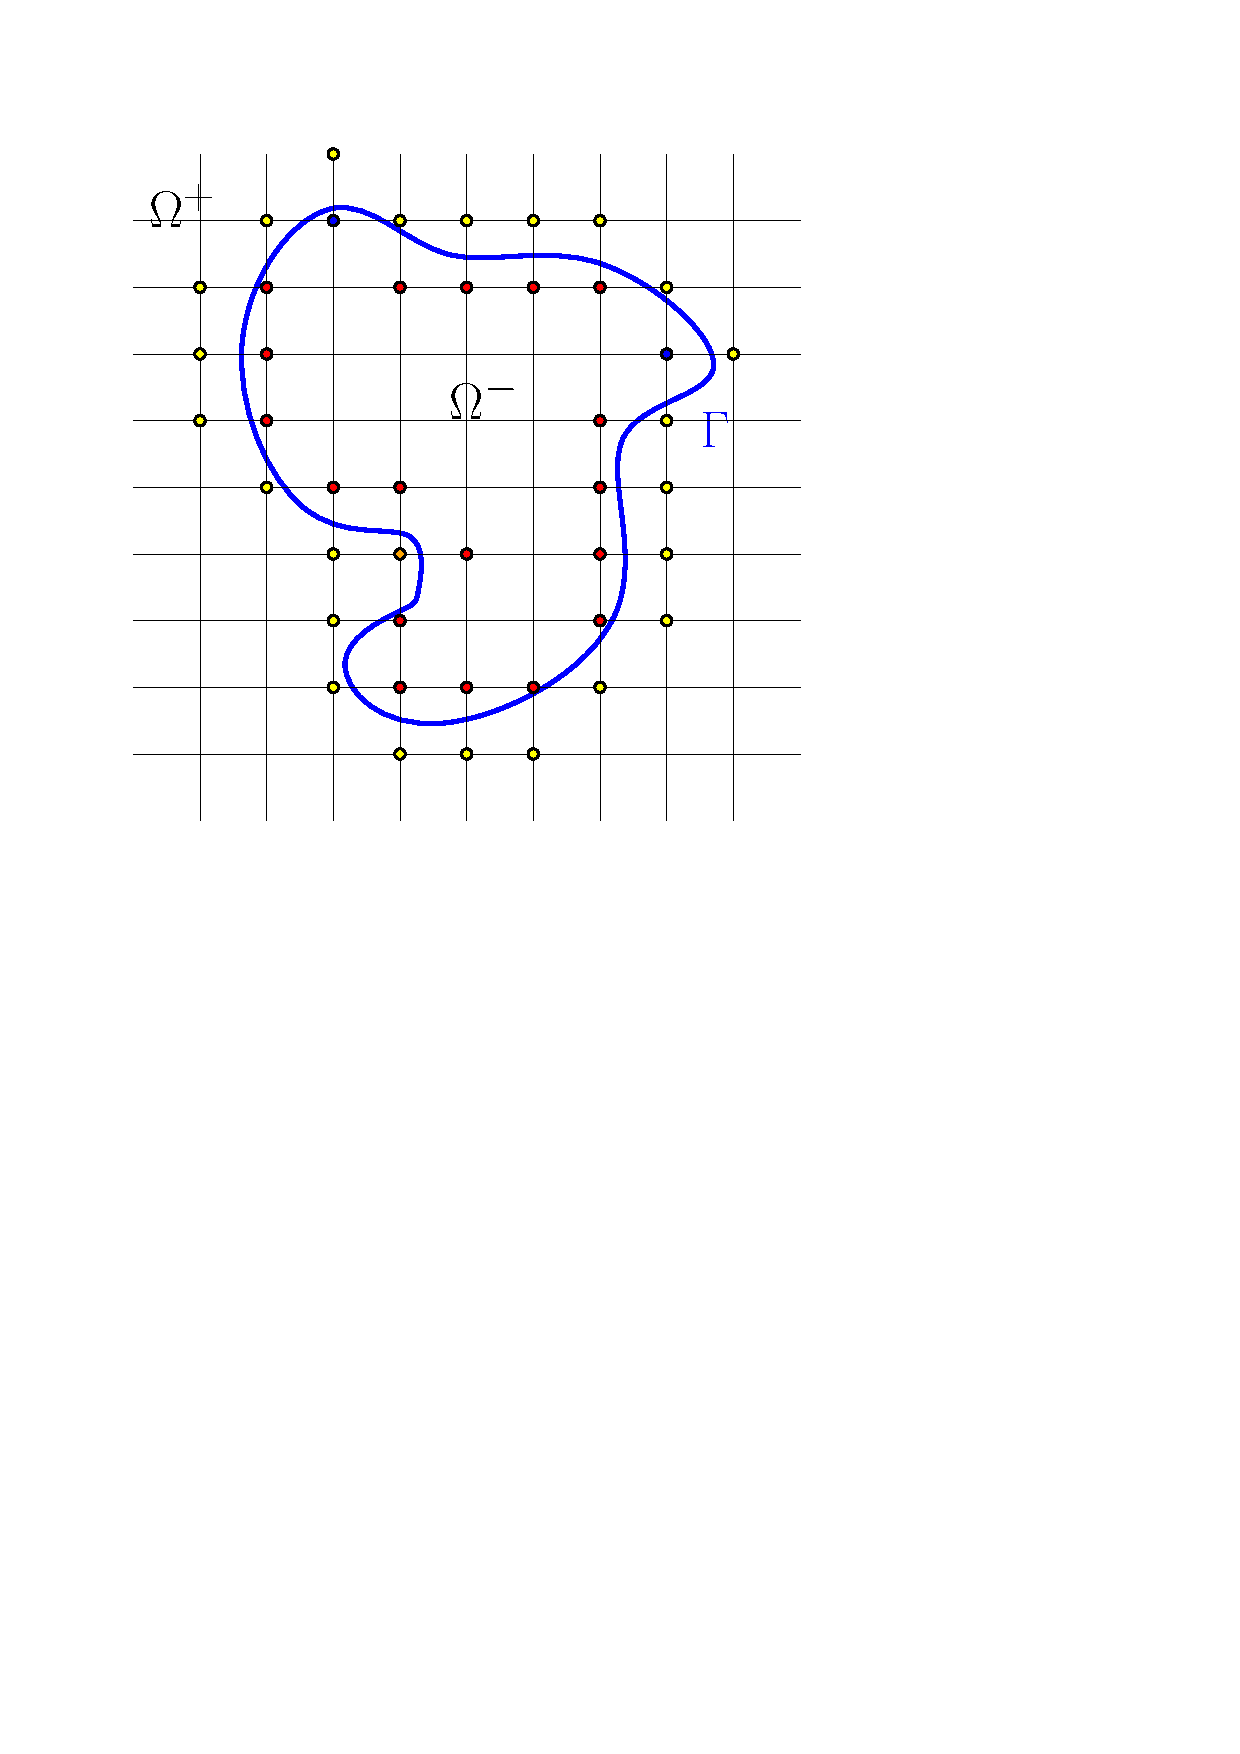
\includegraphics[scale = .7]{PBE1_grid.pdf}
	\caption{Irregular grid points marked as colored disks with blue and orange color for the corner points.}
	\label{fig_irgpoints}
\end{figure}


The Ghost Fluid Method(GFM) is a sharpe interface technique introduced in  \cite{Fedkiw1999} to treat the two-face contact discontinuities in the Euler equations. It extends values across the interface into an artificial fluid (ghost fluid), inducing the jump conditions at the interface. This GFM method was later extended in \cite{Liu2000} to solve elliptic equations with variable coefficients. But in contrast to their method \cite{Liu2000}, the jump conditions are incorporated into the numerical discretization in such a way that the symmetry of the finite difference stencil is preserved. Which makes it compatible with most standard solvers. The flux jump has been decomposed in each axis direction treating the problem dimension by dimension. As a result this extended GFM becomes only first order accurate.   

%%%%%%%%%%%%%%%%%%%%%%%%%%%%%%%%%%%%%%%%%%%%%%%%%%%%%%%%%%%%%%%%%%%%%%%%%%%%%

\section{One dimension}

For a one dimensional representation of the proposed GFM schemes we try to evaluate the finite difference operator $\delta_{xx}$ at the irregular points where the interface is at $x_\Gamma$ between $x_i$ and $x_{i+1}$ as shown in Figure \ref{fig_1}.  %$x_i \leq x_\Gamma\leq x_{i+1}$.   
\begin{figure}[ht]
\begin{center}
%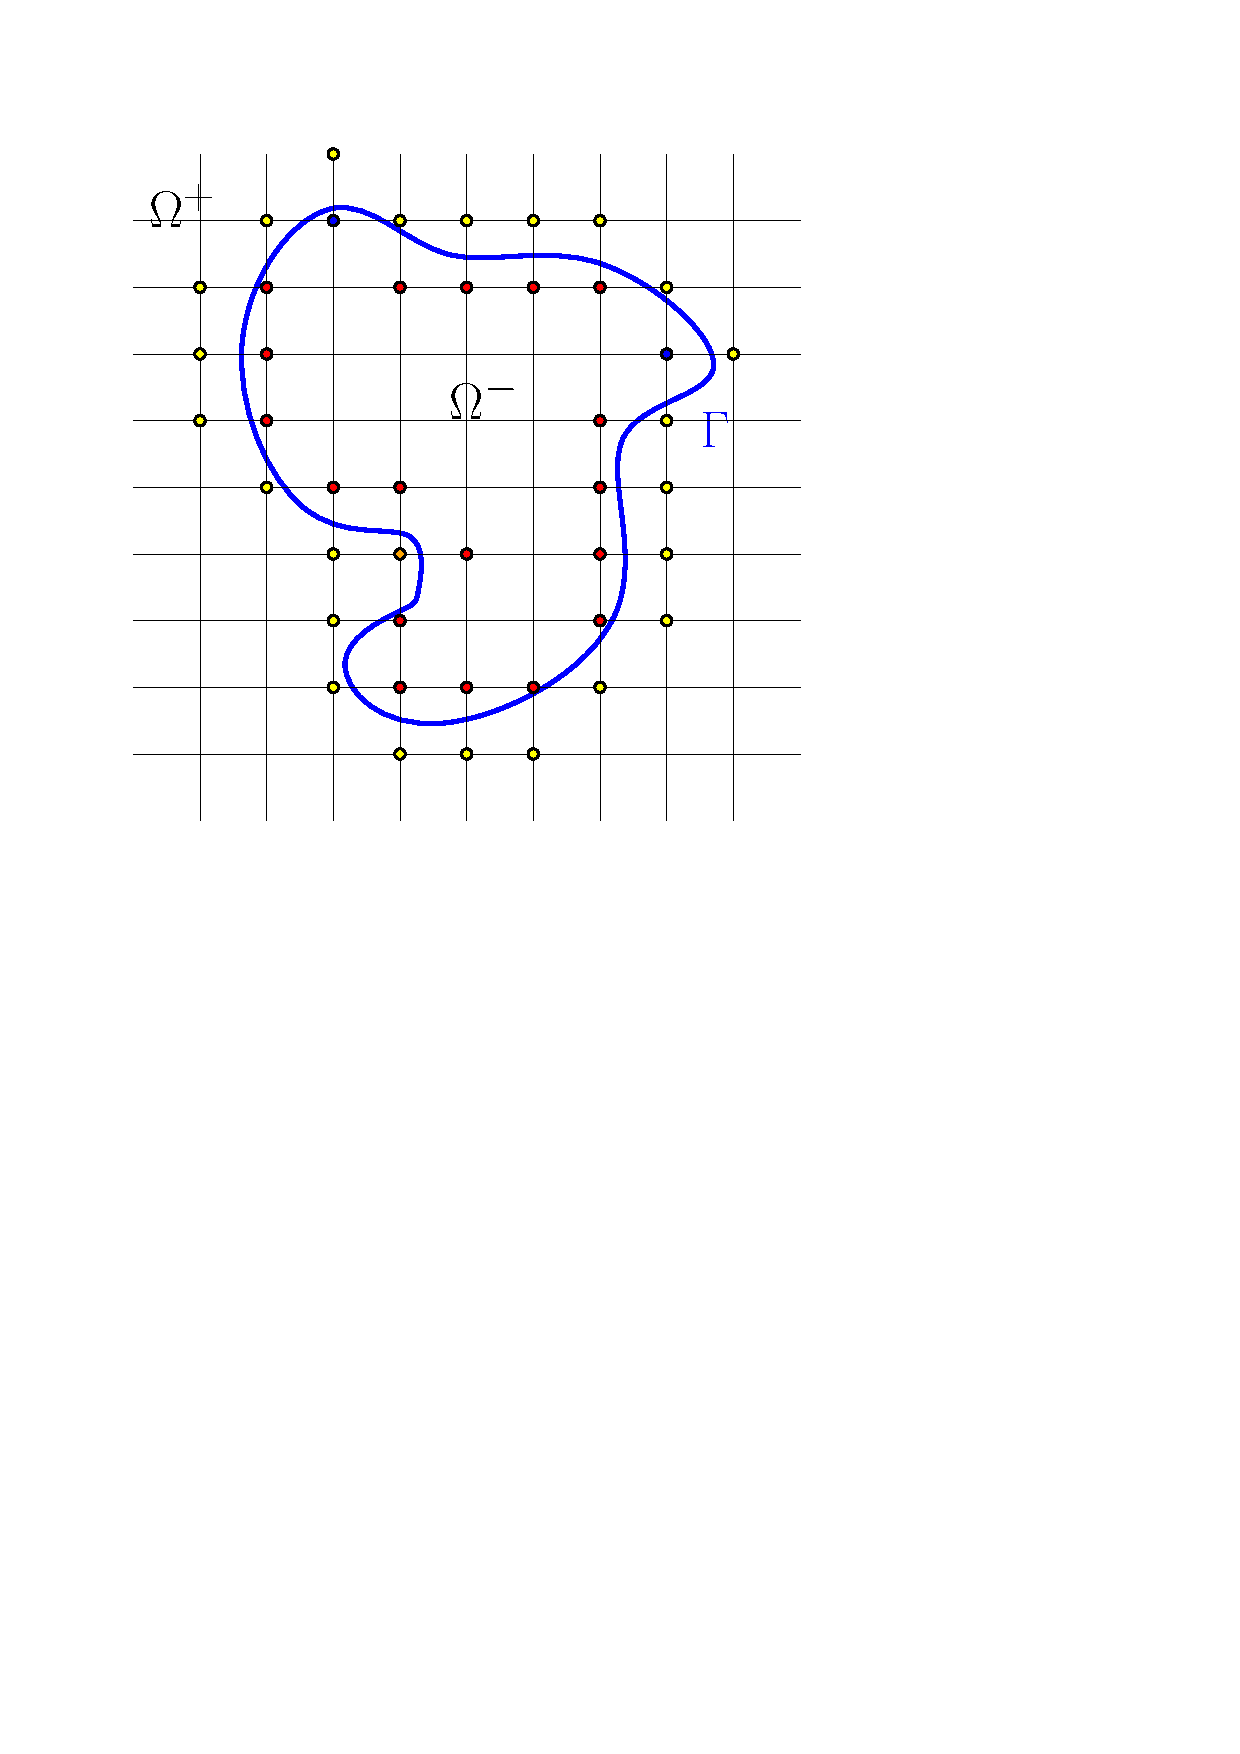
\includegraphics[scale = .5]{PBE1_grid.pdf}
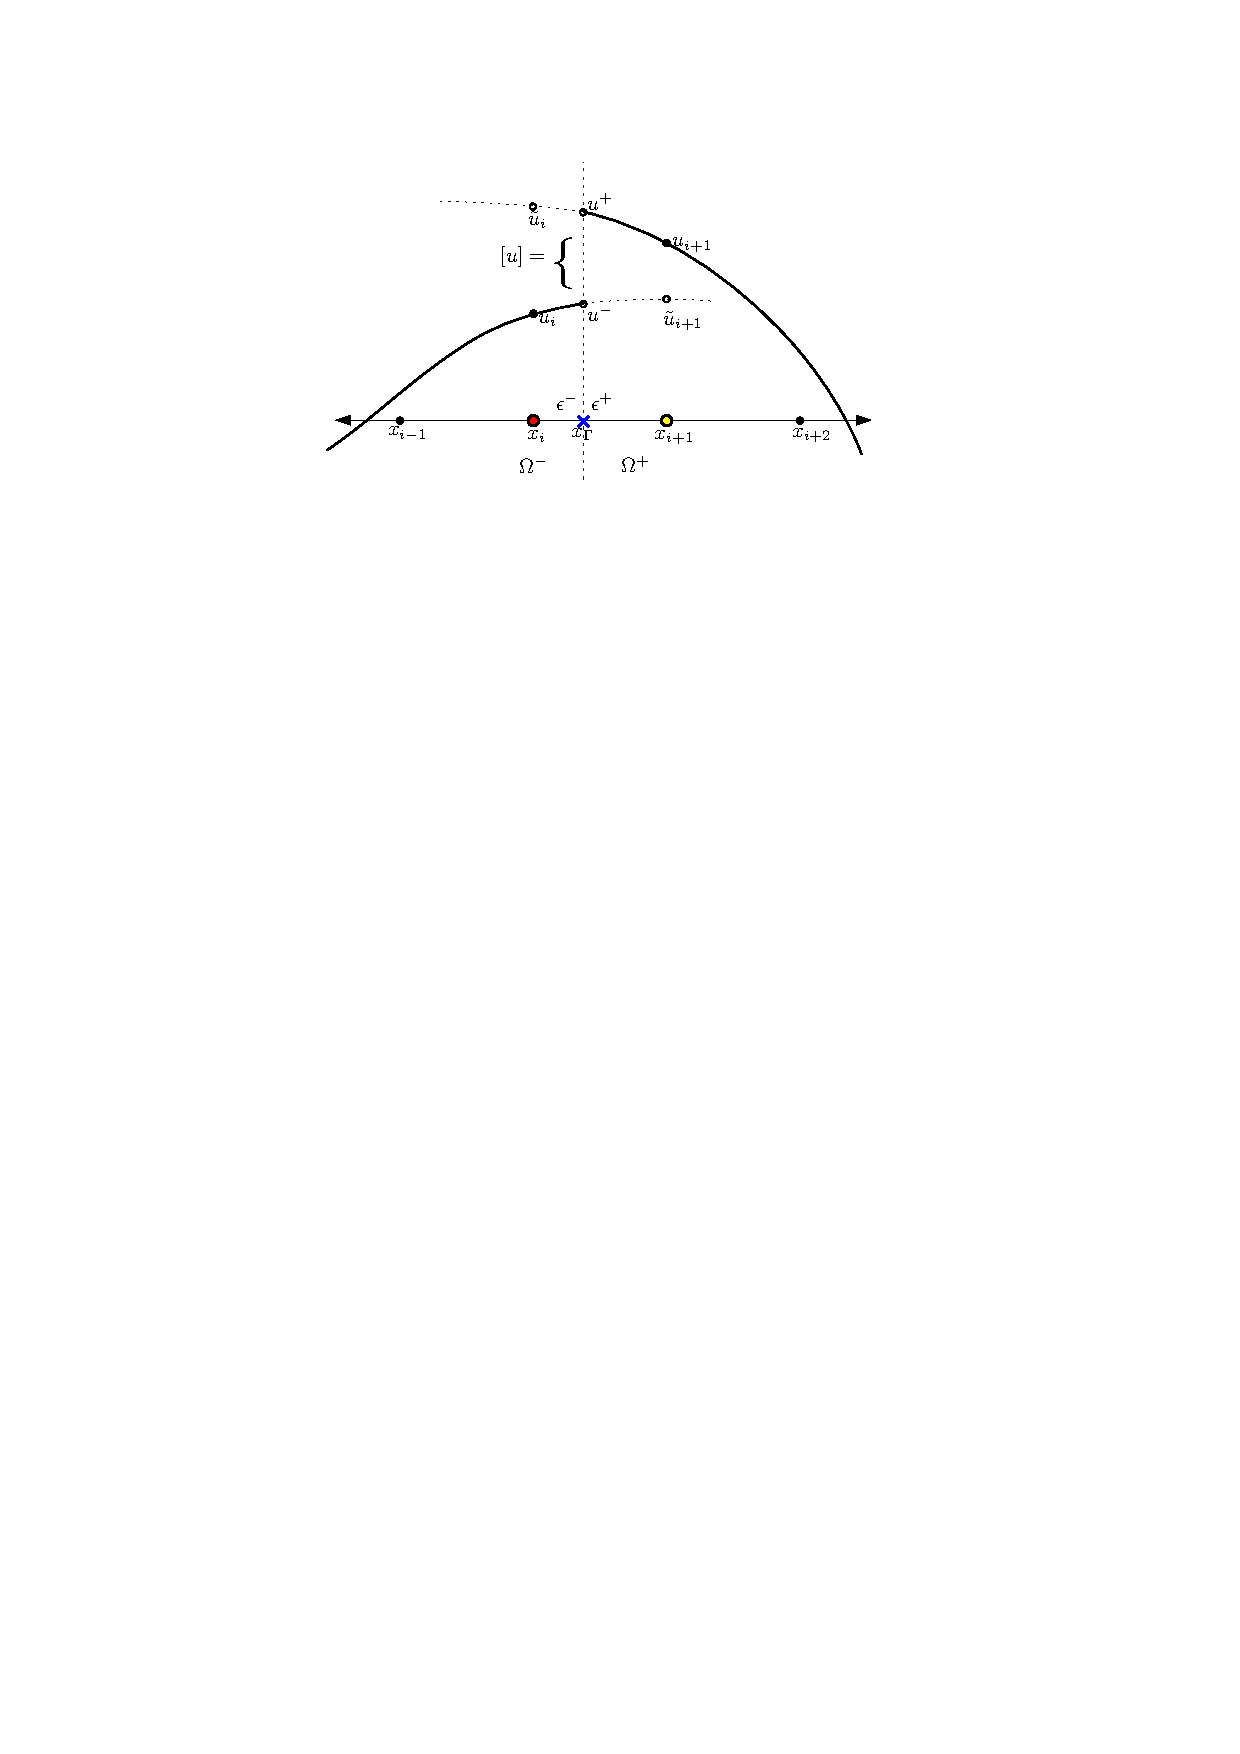
\includegraphics[scale=1.5]{1dmib1.pdf}\hspace{10mm}
\caption{1D GFM. Red and Blue colored points are the irregular points.}
\label{fig_1}
\end{center}
\end{figure}

Here $u$ satisfies the PBE as $u=\begin{cases}
u_{in} \text{ in }\Omega^-\\
u_{out}\text{ in }\Omega^+\\
\end{cases}$ and we define $u^+ = u_{out}(x_\Gamma),u^- = u_{in}(x_\Gamma),h=x_{i+1}-x_i$ and  $\lambda =\frac{x_\Gamma-x_i}{h}$ to get following equations,
\begin{eqnarray}
\begin{aligned}
x_\Gamma &= x_i + \lambda h,  \\
u^- &= u_i(1-\lambda )+ \tilde{u}_{i+1} \lambda \text{ and }u^+ = \tilde{u}_i(1-\lambda )+ u_{i+1}\lambda,x\\
\left[u\right]  & = u^+-u^- \text{ and }\left[ \epsilon \frac{\partial u}{\partial x} \right] =  \epsilon^+ u^+_x-\epsilon^- u^-_x,
\end{aligned}\label{1d_GFM}
\end{eqnarray}
	
where $\tilde{u_i}$ and $\tilde{u_{i+1}}$ are the fictitious values(or ghost values) of $u$ at the irregular points extending $u_{in}$ or $u_{out}$ on the other side of the interface. In particular as shown in Figure \ref{fig_1},  we have $\tilde{u}_i \approx u_{out}(x_i)$ and $\tilde{u}_{i+1}\approx u_{in}(x_{i+1})$. Here $u_{out}$ has been extended to the point $x_i$ for $\tilde{u_i}$ and $u_{in}$ has been extended to the point $x_{i+1}$ for $\tilde{u_i}$. 

Our purpose here is to apply the non-standard finite difference operator $\delta_x^2$ at $x_i$ and $x_{i+1}$ to get: 
\begin{equation}
\delta_x^2\left(u_{i}\right)= \frac{\epsilon^-}{h^2} \left(u_{i-1}-2u_{i}+\tilde{u}_{i+1}\right)\text{ and }\delta_x^2\left(u_{i+1}\right)= \frac{\epsilon^+}{h^2} \left(\tilde{u}_{i}-2u_{i+1}+u_{i+2}\right).	\label{fnt-op}
\end{equation}
Now solving the above equations in (\ref{1d_GFM})  for $\tilde{u}_i $ and $\tilde{u}_{i+1}$ we get, 
\begin{eqnarray}	\tilde{u}_i&=& \frac{\epsilon^-}{\epsilon^+\lambda+\epsilon^-(1-\lambda)}u_i +\frac{\lambda(\epsilon^+-\epsilon^-)}{\epsilon^+\lambda+\epsilon^-(1-\lambda)}u_{i+1}\nonumber\\ &+&\frac{\epsilon^-}{\epsilon^+\lambda+\epsilon^-(1-\lambda)}\left[u\right] -\frac{h \lambda}{\epsilon^+\lambda+\epsilon^-(1-\lambda)}\left[ \epsilon \frac{\partial u}{\partial x} \right]
\end{eqnarray}
and 
\begin{eqnarray}		
	\tilde{u}_{i+1}&=& \frac{(\epsilon^--\epsilon^+)(1-\lambda)}{\epsilon^+\lambda+\epsilon^-(1-\lambda)} u_i +\frac{\epsilon^+}{\epsilon^+\lambda+\epsilon^-(1-\lambda)} u_{i+1}\nonumber \\
	&-&\frac{\epsilon^+}{\epsilon^+\lambda+\epsilon^-(1-\lambda)} \left[u\right] -\frac{h(1-\lambda)}{\epsilon^+\lambda+\epsilon^-(1-\lambda)}\left[ \epsilon \frac{\partial u}{\partial x} \right].\label{u_fact}
\end{eqnarray}
Then substituting equation (\ref{u_fact}) into equation (\ref{fnt-op}) we get
\begin{equation}
		\delta_x^2\left(u_{i}\right)= \frac{1}{h^2} \left(a_1u_{i-1}+b_1 u_{i}+c_1u_{i+1}\right)+\frac{\epsilon^-}{h^2}\left(e_1.[u]+f_1.\left[ \epsilon \frac{\partial u}{\partial x} \right]\right)\label{fnt-op-1}
\end{equation}
and 
\begin{equation}		
		\delta_x^2\left(u_{i+1}\right)= \frac{1}{h^2} \left(a_2u_{i}-b_2u_{i+1}+c_2u_{i+2}\right)+\frac{\epsilon^+}{h^2}\left(e_2.[u]+f_2.\left[ \epsilon \frac{\partial u}{\partial x} \right]\right)\label{fnt-op-2}
\end{equation}
where,
\begin{eqnarray}
\begin{aligned}
d&=\epsilon^+\lambda+\epsilon^-(1-\lambda),\\
a_1&= \epsilon^-,b_1=-\epsilon^-\left(1+\frac{\epsilon^+}{d}\right), c_1=\frac{\epsilon^-\epsilon^+}{d}, e_1=\frac{\epsilon^-}{d},f_1=\frac{h\lambda}{d},\\
a_2&= \frac{\epsilon^+\epsilon^-}{d},b_2=-\epsilon^+\left(1+\frac{\epsilon^-}{d}\right), c_2=\epsilon^+, e_2=-\frac{\epsilon^+}{d},f_2=\frac{h(1-\lambda)}{d}.
\end{aligned}
\end{eqnarray}
Here, the second terms of the equations in (\ref{fnt-op-2}) are known. Only the coefficients in the 1st terms of (\ref{fnt-op-2}) contribute to the finite difference operator matrix keeping it tridiagonal to make it diagonally dominant(as $|b_1|-a_1-c_1=0\text{ and } |b_2|-a_2-c_2=0$) and symmetric (as $a_2=c_1$).  
%%%%%%%%%%%%%%%%%%%%%%%%%%%%%%%%%%%%%%%%%%%%%%%%%%%%%%%%%%%%%%%%%%%%%%%%%%%%%

  
\section{Two dimensions}
For the two dimensional PB model, we need to evaluate $\delta_{xx}$ and $\delta_{yy}$, 
where $\delta_{yy}$ can be calculated at irregular points in a manner similar to (\ref{fnt-op-2}) 
%where the similar derivation of the equations in (\ref{fnt-op-2}) can be used to calculate $\delta_{yy}$ at irregular points. 
In this case,  $\left[ \epsilon \frac{\partial u}{\partial x} \right]$ and $\left[ \epsilon \frac{\partial u}{\partial y} \right]$ are not known, while $\left[ \epsilon \frac{\partial u}{\partial n} \right]$ is given. Now to get $\left[ \epsilon \frac{\partial u}{\partial x} \right]$ and $\left[ \epsilon \frac{\partial u}{\partial y} \right]$ in terms of $\left[ \epsilon \frac{\partial u}{\partial n} \right]$ and $\left[ \epsilon \frac{\partial u}{\partial \tau} \right]$ we have the following relations,  
\begin{figure}[ht]
\begin{center}
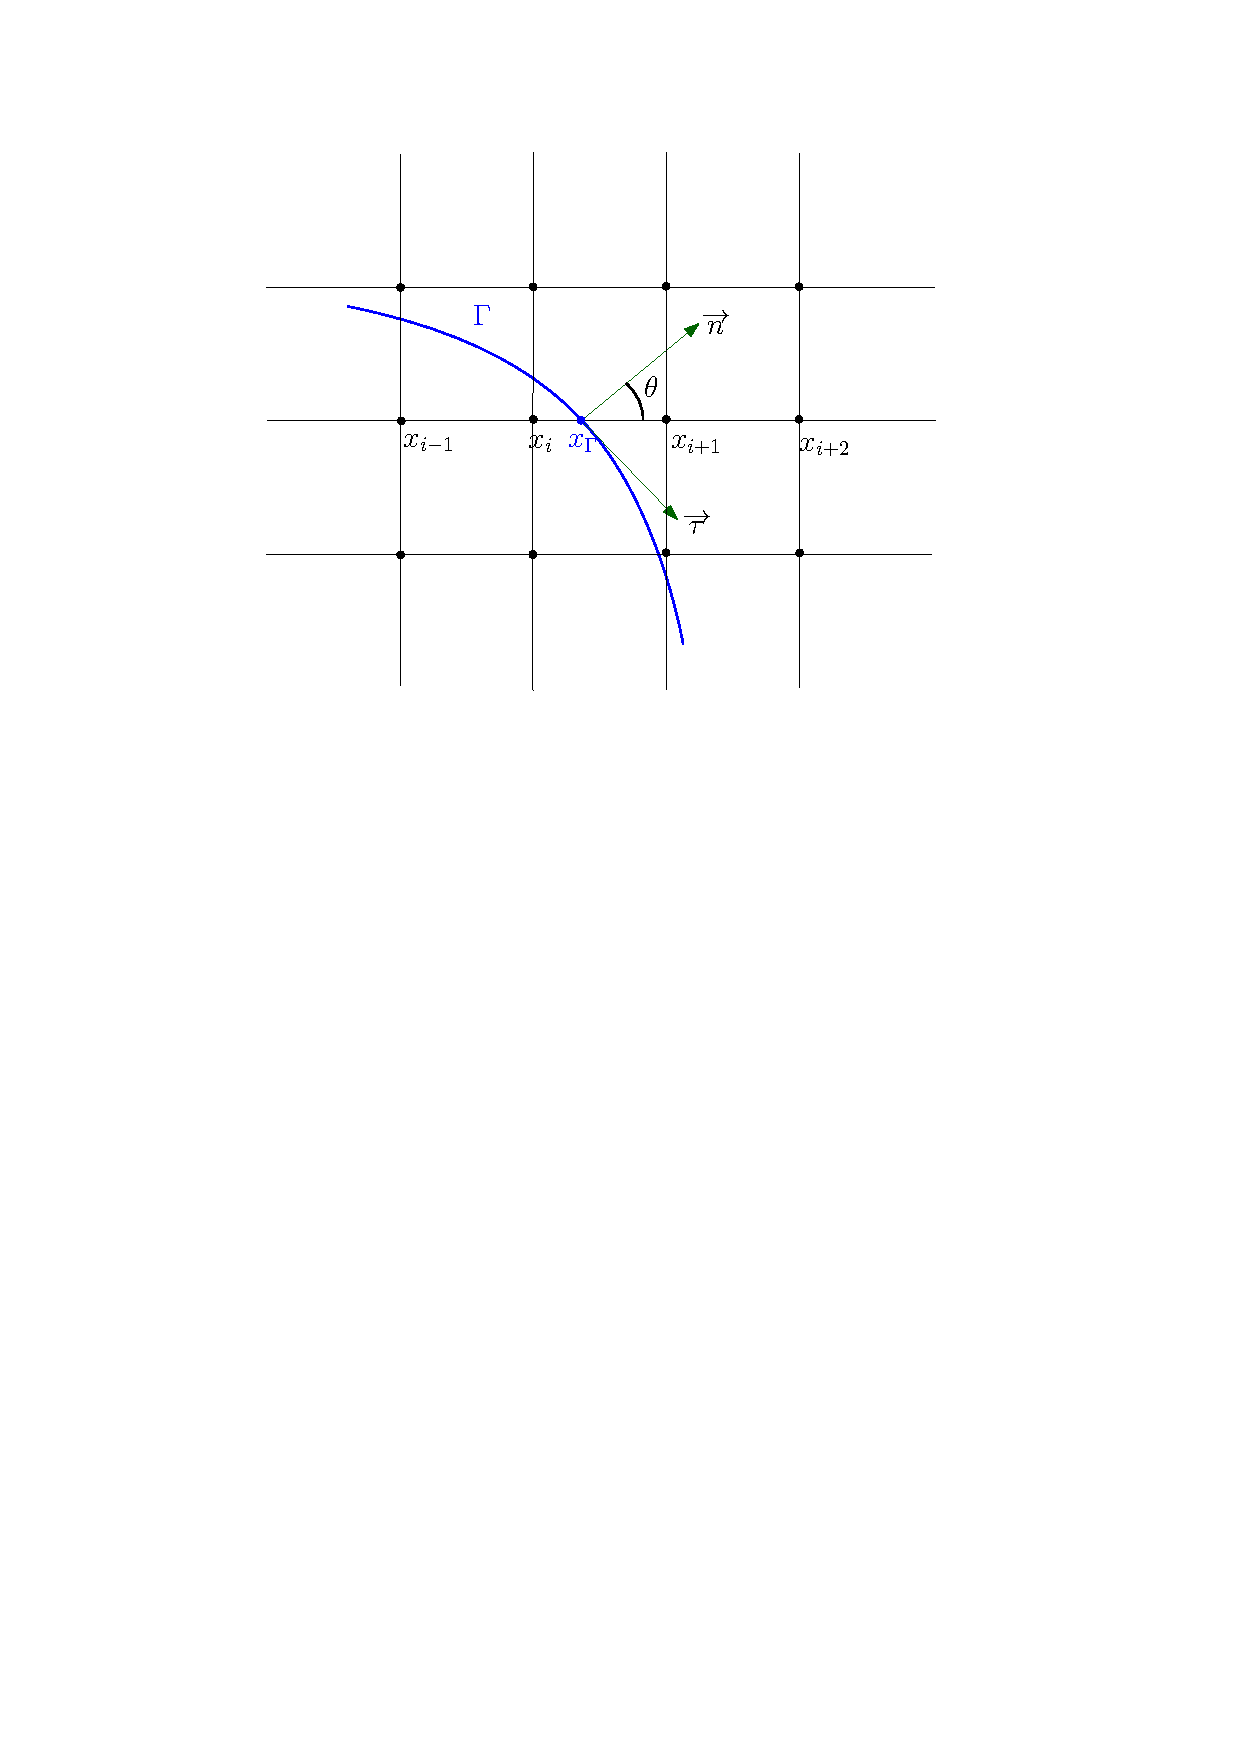
\includegraphics[width = 0.7\textwidth ]{GFM_2D.pdf}
\caption{2D GFM with the interface $\Gamma$ and the normal direction $\vec{n}$.}
\label{fig_gfm_2D}
\end{center}
\end{figure}

\begin{eqnarray}
\begin{aligned}
			\left[\epsilon \frac{\partial u}{\partial n}\right] &=& \cos \theta \left[\epsilon \frac{\partial u}{\partial x}\right] + sin \theta \left[\epsilon \frac{\partial u}{\partial y}\right],\label{epun} \\
			\left[\epsilon \frac{\partial u}{\partial \tau}\right] &=& sin \theta \left[\epsilon \frac{\partial u}{\partial x}\right] - \cos \theta\left[\epsilon \frac{\partial u}{\partial y}\right],\label{eput}	
\end{aligned}		
\end{eqnarray}
where $\theta$ is the angle between the normal direction and positive $x$ direction, as shown in Figure \ref{fig_gfm_2D}. 
Equation \ref{eput} can be solved for $ \left[\epsilon \frac{\partial u}{\partial x}\right]$ and $\left[\epsilon \frac{\partial u}{\partial y}\right]$:
\begin{eqnarray}
\begin{aligned}
	\left[\epsilon \frac{\partial u}{\partial x}\right] &=& \cos \theta \left[\epsilon \frac{\partial u}{\partial n}\right] +sin \theta \left[\epsilon \frac{\partial u}{\partial \tau}\right],\label{epux1} \\
	\left[\epsilon \frac{\partial u}{\partial y}\right] &=& sin \theta \left[\epsilon \frac{\partial u}{\partial n}\right] -\cos \theta \left[\epsilon \frac{\partial u}{\partial \tau}\right].\label{epuy1}
\end{aligned}	
\end{eqnarray}
To simplify the jump-conditions Liu, Fedkiw and Kang \cite{Liu2000}  smeared out the tangential derivative by considering $\left[\epsilon \frac{\partial u}{\partial \tau}\right]=0$ to get the following equations, 
%		\begin{eqnarray}
%			\left[\epsilon u_x\right] &=& \cos \theta \left[\epsilon u_n\right] \label{epux2}  \\
%			\left[\epsilon u_y\right] &=& sin \theta \left[\epsilon u_n\right] \label{epuy2}
%		\end{eqnarray}
\begin{eqnarray}
\begin{aligned}
	\left[\epsilon \frac{\partial u}{\partial x}\right] &\approx& \cos \theta \left[\epsilon \frac{\partial u}{\partial n}\right],\label{epux2}   \\
	\left[\epsilon \frac{\partial u}{\partial y}\right] &\approx& \sin \theta \left[\epsilon \frac{\partial u}{\partial n}\right], \label{epuy2}
\end{aligned}	
\end{eqnarray}
which are in general not true.
% but $\left[\epsilon \frac{\partial u}{\partial x}\right]$ and $\left[\epsilon \frac{\partial u}{\partial y}\right]$ in (\ref{epux2}) satisfies (\ref{epun}) for $\left[\epsilon \frac{\partial u}{\partial n}\right]$. 
It allows us to replace the unknown quantities as  $\left[\epsilon \frac{\partial u}{\partial x}\right]$ and $\left[\epsilon \frac{\partial u}{\partial y}\right]$ by the known quantities $\left[\epsilon \frac{\partial u}{\partial n}\right]$ and $\left[\epsilon \frac{\partial u}{\partial \tau}\right]$. This process used to simplify the jump condition in \cite{Liu2000} still requires the normal direction $\theta$. In our proposed GFM scheme  we have considered $\frac{\partial u^+}{\partial \tau}=0$ to get the following derivation for $ \left[\epsilon \frac{\partial u}{\partial x}\right] $:
\begin{eqnarray*}
\left[\epsilon \frac{\partial u}{\partial x}\right] &=& \cos \theta \left[\epsilon \frac{\partial u}{\partial n}\right] +\sin \theta \left[\epsilon \frac{\partial u}{\partial \tau}\right]\\
&=& \cos \theta \left[\epsilon \frac{\partial u}{\partial n}\right] +\sin \theta \left(\epsilon^+\frac{\partial u^+}{\partial \tau}-\epsilon^-\frac{\partial u^-}{\partial \tau}\right)\\
&=& \cos \theta\left[\epsilon \frac{\partial u}{\partial n}\right]+\sin \theta \left(\epsilon^+\frac{\partial u^+}{\partial \tau}-\epsilon^-\frac{\partial u^+}{\partial \tau}+\epsilon^-\frac{\partial u^+}{\partial \tau}-\epsilon^-\frac{\partial u^-}{\partial \tau}\right)\\
&=&\cos \theta\left[\epsilon \frac{\partial u}{\partial n}\right]+\sin \theta \left(\epsilon^-\left(\frac{\partial u^+}{\partial \tau}-\frac{\partial u^-}{\partial \tau}\right)+(\epsilon^+-\epsilon^-)\frac{\partial u^+}{\partial \tau}\right)\\
&=&\cos \theta\left[\epsilon \frac{\partial u}{\partial n}\right]+\sin \theta \left(\epsilon^-\left[\frac{\partial u}{\partial \tau}\right]+(\epsilon^+-\epsilon^-)\frac{\partial u^+}{\partial \tau}\right)
\end{eqnarray*}
Now by the jump conditions we have $ \left[\epsilon \frac{\partial u}{\partial n}\right] =\epsilon^- \frac{\partial G}{\partial n}$ and $\left[\frac{\partial u}{\partial \tau}\right]= \frac{\partial G}{\partial \tau}.$
\begin{eqnarray*}
\text{Thus } \left[\epsilon \frac{\partial u}{\partial x}\right] &=& \cos \theta (\epsilon^- \frac{\partial G}{\partial n})+\sin \theta .\epsilon^- \frac{\partial G}{\partial \tau} +\sin \theta (\epsilon^+ -\epsilon^- ) \frac{\partial u^+}{\partial \tau}\\
&\approx & \epsilon^-(\cos \theta  \frac{\partial G}{\partial n}+\sin \theta\frac{\partial G}{\partial \tau}) = \epsilon^- \frac{\partial G}{\partial x}\text{, if }\frac{\partial u^+}{\partial \tau}=0.\\
\text{Therefore, }\left[\epsilon \frac{\partial u}{\partial x}\right]&\approx &  \epsilon^- \frac{\partial G}{\partial x}.
\end{eqnarray*}
Similarly it can be shown that $\left[\epsilon \frac{\partial u}{\partial y}\right] \approx   \epsilon^- \frac{\partial G}{\partial y}$. Like the original GFM, our new GFM also omits some tangential information. Thus, two methods will have a local first order of truncation error. Nevertheless, in our new method, the normal direction of the complicated molecular surface is not required, so that the implementation of the modified GFM is much simpler than the standard GFM. 

%Now using  $\left[ u\right]= G$ from (\ref{phitilde3}) and $\left[\epsilon\frac{\partial u}{\partial x}\right]= \epsilon^-\frac{\partial G}{\partial x}$ from (\ref{phitilde4}) as the jump condition we have,
%%\begin{eqnarray}
%%	u^+-u^- &=& G\\
%%	\epsilon^+ u^+_x-\epsilon^- u^-_x &=& \epsilon^-\frac{\partial G}{\partial x}
%%\end{eqnarray}
%\begin{align*}
%	\tilde{u}_i&= \frac{\epsilon^-}{\epsilon^+\lambda+\epsilon^-(1-\lambda)}\textcolor{blue}{u_i} +\frac{\lambda(\epsilon^+-\epsilon^-)}{\epsilon^+\lambda+\epsilon^-(1-\lambda)}\textcolor{blue}{u_{i+1}}\\
%	&+\frac{\epsilon^-}{\epsilon^+\lambda+\epsilon^-(1-\lambda)} \textcolor{blue}{G}-\frac{h \lambda}{\epsilon^+\lambda+\epsilon^-(1-\lambda)}\textcolor{blue}{\epsilon^- \frac{\partial G}{\partial x}}\\
%	\tilde{u}_{i+1}&= \frac{(\epsilon^--\epsilon^+)(1-\lambda)}{\epsilon^+\lambda+\epsilon^-(1-\lambda)} \textcolor{blue}{u_i} +\frac{\epsilon^+}{\epsilon^+\lambda+\epsilon^-(1-\lambda)} \textcolor{blue}{u_{i+1}}\\
%	& -\frac{\epsilon^+}{\epsilon^+\lambda+\epsilon^-(1-\lambda)} \textcolor{blue}{G}-\frac{h(1-\lambda)}{\epsilon^+\lambda+\epsilon^-(1-\lambda)}\textcolor{blue}{ \epsilon^-\frac{\partial G}{\partial x}}
%\end{align*}


%%%%%%%%%%%%%%%%%%%%%%%%%%%%%%%%%%%%%%%%%%%%%%%%%%%%%%%%%%%%%%%%%%%%%%%%%%%%%

\section{Three dimensions}

Consider that the interface $\Gamma$ that intersects the grid line in the $x$ direction at a point $(i_\Gamma, j,k)$ which is located between $(i,j,k)$ and $(i+1,j,k)$, We therefore have two irregular grid points, $(i,j,k)$ and $(i+1,j,k)$. The fictitious values $\tilde{u}_{i,j,k}$ and $\tilde{u}_{i+1,j,k}$ are to be determined. To use one of the jump conditions which is defined in the normal direction of the interface point, it is convenient to introduce a local coordinates $(\xi,\eta,\zeta)$ such that $\xi$ is along the normal direction and $\eta $ is in the $xy$ plane. Then the coordinate transformation can be given as, 
\begin{align}
  \left[
            \begin{array}{c}
             x\\
             y\\
             z
       \end{array}\right] =\bf{P}\left[\begin{array}{c}
            \xi\\
            \eta\\
            \zeta
     \end{array}\right],\label{eqtran1}
\end{align}
%\begin{align}
%    \left[\begin{array}{c}
%            \xi\\
%            \eta\\
%            \zeta
%     \end{array}\right]=\bf{P}\left[
%            \begin{array}{c}
%             x\\
%             y\\
%             z
%       \end{array}\right],\label{eqtran1}
%\end{align}
where $\bf{P}$ is the transformation matrix
%\begin{align}
%    \bf{P}=\left[\begin{array}{ccc}
%                 \sin\psi\cos\theta & \sin\psi\sin\theta & \cos\psi\\
%                 -\sin\theta        & \cos\theta         & 0       \\
%                 -\cos\psi\cos\theta&-\cos\psi\sin\theta & \sin\psi
%                 \end{array}\right]. \label{eqtran2}
%\end{align}
\begin{align}
    \bf{P}=\left[\begin{array}{ccc}
                 \sin\psi\cos\theta  &-\sin\theta   & -\cos\psi\cos\theta \\
                \sin\psi\sin\theta   & \cos\theta   & -\cos\psi\sin\theta \\
                  \cos\psi 			 & 0 			& \sin\psi
                 \end{array}\right]. \label{eqtran2}
\end{align}
Here $\theta$ and $\psi $ are the azimuth and zenith angles with respect to the normal direction $\xi$.
% Now to express the jump condition along x-axis $\left[\epsilon \frac{\partial u}{\partial x}\right]$  in terms of $\left[\epsilon \frac{\partial u}{\partial \xi}\right]$, $\left[\epsilon \frac{\partial u}{\partial \eta}\right]$ and $\left[\epsilon \frac{\partial u}{\partial \zeta}\right]$ we have 
Then from equation (\ref{eqtran1}) and (\ref{eqtran2}) we have, 
\begin{eqnarray}
	\left[\epsilon \frac{\partial u}{\partial x}\right] &=& \sin \psi \cos \theta \left[\epsilon \frac{\partial u}{\partial \xi}\right]-\sin \theta \left[\epsilon \frac{\partial u}{\partial \eta}\right]-\cos \psi \cos \theta \left[\epsilon \frac{\partial u}{\partial \zeta}\right]\label{3d_gfm1}
\end{eqnarray}
Now along the $\eta$ axis,
\begin{eqnarray}
\begin{aligned}
	\left[\epsilon \frac{\partial u}{\partial \eta}\right] &= \epsilon^+\frac{\partial u^+}{\partial \eta }-\epsilon^-\frac{\partial u^-}{\partial \eta }\\
	&=\epsilon^+\frac{\partial u^+}{\partial \eta }-\epsilon^-\frac{\partial u^+}{\partial \eta }+\epsilon^-\frac{\partial u^+}{\partial \eta }-\epsilon^-\frac{\partial u^-}{\partial \eta }\\
	&= \epsilon^-\left(\frac{\partial u^+}{\partial \eta }-\frac{\partial u^-}{\partial \eta }\right)+(\epsilon^+-\epsilon^-)\frac{\partial u^+}{\partial \eta}\\
	&= \epsilon^-\frac{\partial G}{\partial \eta}+(\epsilon^+-\epsilon^-)\frac{\partial u^+}{\partial \eta}\text{ since } \left(\frac{\partial u^+}{\partial \eta }-\frac{\partial u^-}{\partial \eta }\right)=\frac{\partial}{\partial\eta}[u]=\frac{\partial G}{\partial \eta}.\label{3d_gfm2}
\end{aligned}
\end{eqnarray}
Similarly along the $\zeta $ axis, 
\begin{equation}
	\left[\epsilon \frac{\partial u}{\partial \zeta}\right]= \epsilon^-\frac{\partial G}{\partial \zeta}+(\epsilon^+-\epsilon^-)\frac{\partial u^+}{\partial \zeta }.\label{3d_gfm3}
\end{equation}
Then from equations (\ref{3d_gfm1}), (\ref{3d_gfm2}) and (\ref{3d_gfm3}) we have,
\begin{eqnarray}
\begin{aligned}   
		\left[\epsilon \frac{\partial u}{\partial x}\right]&= \epsilon^-\left( \sin \psi \cos \theta \frac{\partial G}{\partial \xi}-\sin \theta \frac{\partial G}{\partial \eta}-\cos \psi \cos \theta \frac{\partial G}{\partial \zeta}\right)\\
		 &-\sin\theta (\epsilon^+-\epsilon^-)\frac{\partial u}{\partial \eta}^+ -\cos{\phi} \cos \theta (\epsilon^+-\epsilon^-) \frac{\partial u^+}{\partial \zeta }\\
		 &=\epsilon^- \frac{\partial G}{\partial x}-\sin\theta (\epsilon^+-\epsilon^-)\frac{\partial u}{\partial \eta}^+ -\cos{\phi} \cos \theta (\epsilon^+-\epsilon^-) \frac{\partial u^+}{\partial \zeta }\\
		 &\approx \epsilon^- \frac{\partial G}{\partial x}\text{     assuming } \frac{\partial u}{\partial \eta}^+ =0 \text{ and } \frac{\partial u^+}{\partial \zeta }=0.  
\end{aligned}\label{eq:m-gfm1}		  	
\end{eqnarray}
Similarly along $y$ axis and $z$ axis from equation (\ref{3d_gfm1}),(\ref{3d_gfm2}) and (\ref{3d_gfm3}) we have:
\begin{eqnarray}
\begin{aligned}  
\left[\epsilon \frac{\partial u}{\partial y}\right]\approx\epsilon^- \frac{\partial G}{\partial y}\text{ and } \left[\epsilon \frac{\partial u}{\partial z}\right]\approx\epsilon^- \frac{\partial G}{\partial z}.\label{eq:m-gfm2}
\end{aligned}		  	
\end{eqnarray}
%%%%%%%%%%%%%%%%%%%%%%%%%%%%%%%%%%%%%%%%%%%%%%%%%%%%%%%%%%%%%%%%%%%%%%%%%%%%%

\section{Corner point for the modified GFM method}
% TODO Maybe have to describe more about Corner point
We have a special situation for a corner point when the interface crosses the grid line for the same axis twice around $x_i$ where $x_{i-1}$ and $x_{i+1}$ are on the other side of the interface as shown in Figure \ref{fig:corner_point}. There are two types of corner point situations. In one type the point $x_i$ is in $\Omega^-$ and the other two adjacent points are in $\Omega^+$ (see Figure \ref{fig:corner_point}). For this case we define $G_L=-G$ and $G_R = G$ to derive the following equations for the fictitious points $\tilde{u}_{i-1}$ and $\tilde{u}_{i+1}$: 
\begin{figure}[!h]		
\begin{center}
	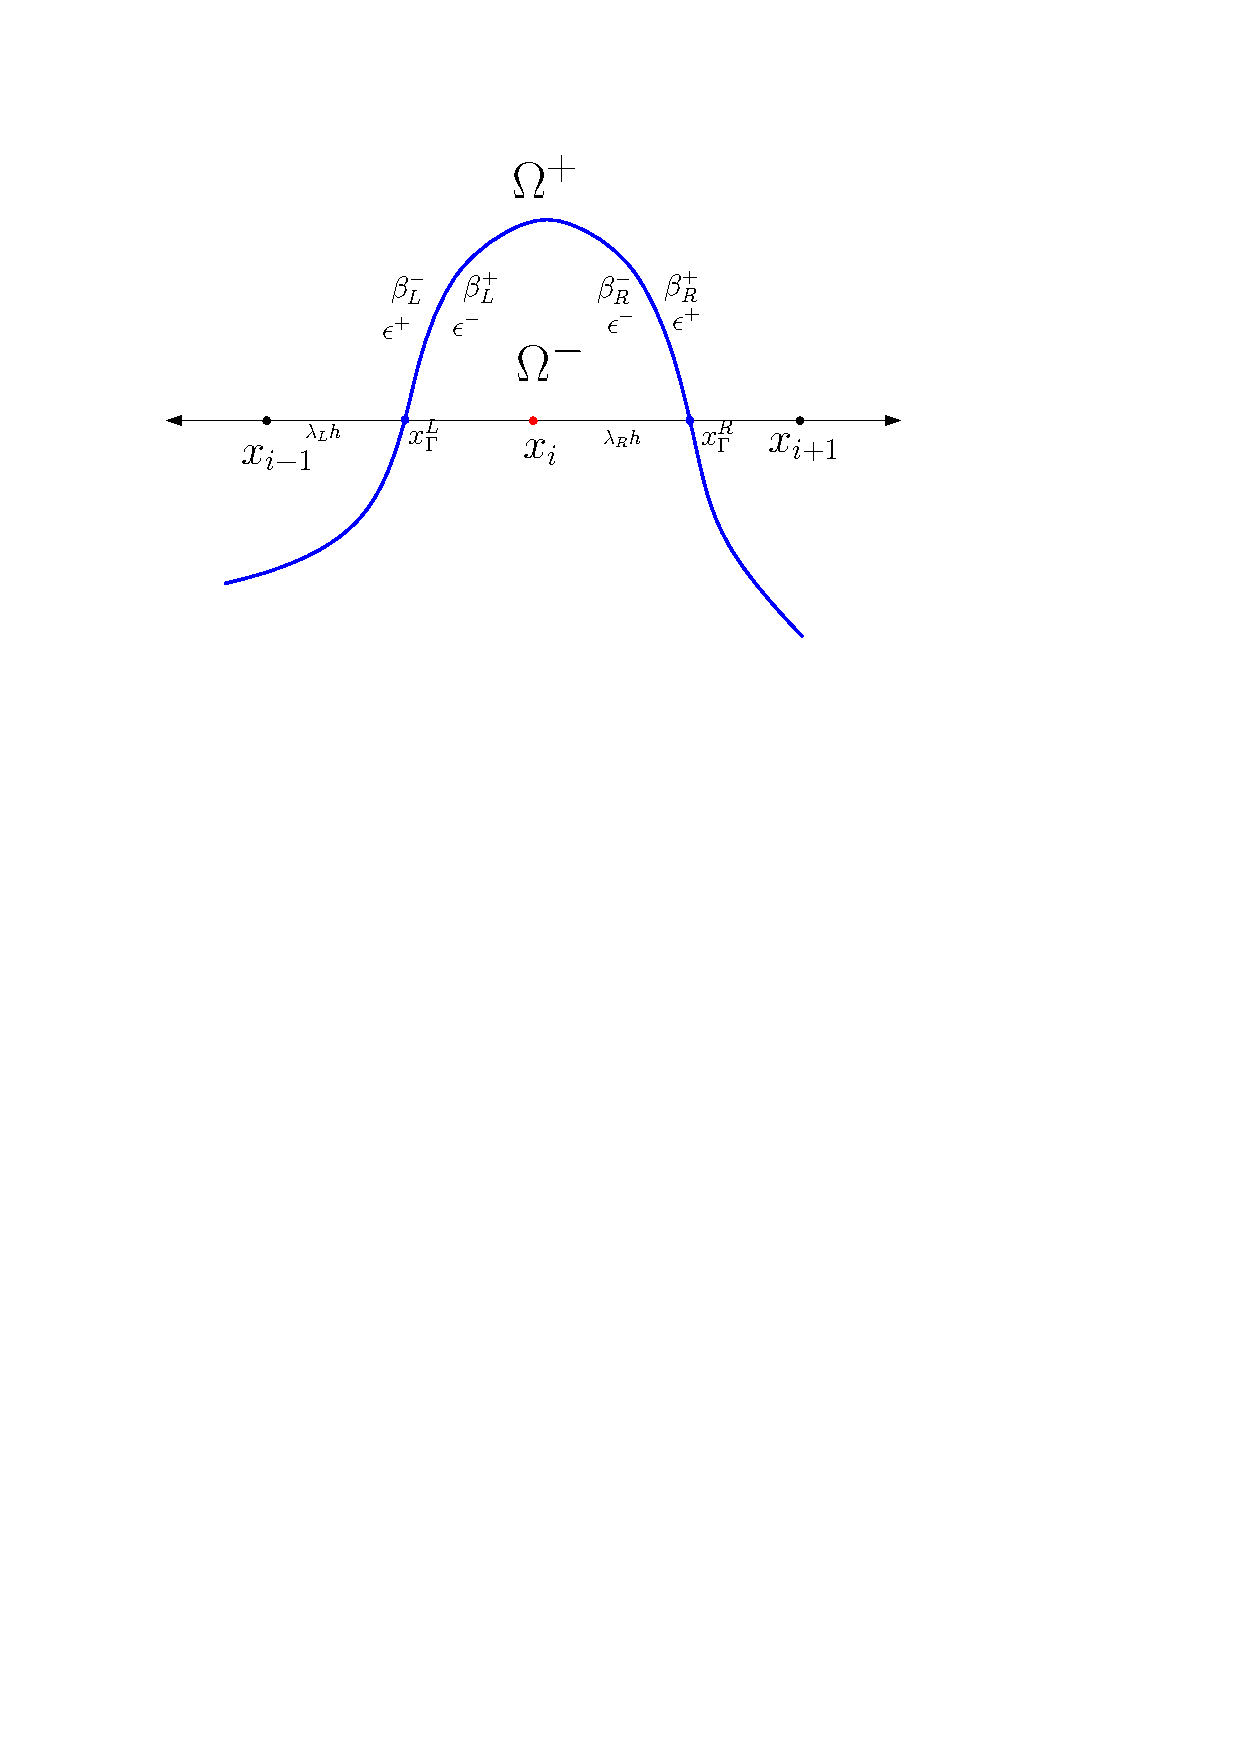
\includegraphics[width = 0.7\textwidth ]{GFMcorner.pdf}		
\end{center}
\caption{2D representation for a corner point treatment for the point $x_i$ }
\label{fig:corner_point}
\end{figure}
\begin{equation}
	\tilde{u}_{i-1}= A_1 u_{i-1}+B_1 u_{i} + C_1 G_L- D_1 \epsilon^- \frac{\partial G_L}{\partial x},\label{eq:corner1}
\end{equation}
and
\begin{equation}	
	\tilde{u}_{i+1}= A_2 u_{i+1}+B_2 u_{i} - C_2 G_R- D_2 \epsilon^- \frac{\partial G_R}{\partial x},\label{eq:corner2}
\end{equation}
where,
    $$	A_1 = \frac{\beta^-_L}{F_1}, B_1  = \frac{\lambda_L(\beta^+_L-\beta^-_L)}{F_1}, C_1 = \frac{\beta^-_L}{F_1},D_1 = \frac{h \lambda_L}{F_1}, $$ %, 
	$$A_2 = \frac{\beta^+_R}{F_2}, B_2  = \frac{(1-\lambda_R)(\beta^-_R-\beta^+_R)}{F_2}, C_2 = \frac{\beta^+_R}{F_2},D_2 = \frac{h(1- \lambda_R)}{F_2},$$
	$$\beta_L^-=\epsilon^+,\beta_L^+=\epsilon^-,\beta_R^-=\epsilon^-,\beta_R^+=\epsilon^+,$$
	$$\lambda_L=\frac{x^L_\Gamma-x_{i-1}}{h},\lambda_R=\frac{x^R_\Gamma-x_i}{h},$$
	$$F_1 = \beta^+_L \lambda_L+\beta^-_L(1-\lambda_L), F_2 = \beta^+_R \lambda_R+\beta^-_R(1-\lambda_R).$$
For the other type of the corner points we have the point $x_i$ in $ \Omega^+$ with its adjacent points in $x$ direction in $\Omega^-$. We can use the similar type of calculation like the previous type of corner points considering $G_L=G$ and $G_R = -G$ to find the factious points using the equations (\ref{eq:corner1}) and (\ref{eq:corner2}). 

	
%%%%%%%%%%%%%%%%%%%%%%%%%%%%%%%%%%%%%%%%%%%%%%%%%%%%%%%%%%%%

\section{Simplicity of the modified GFM}

Altogether this proposed modified GFM is much more easier to program compared to the MIB method used in \cite{Zhihan2017}. Unlike the MIB method, the modified GFM doesn't need to generate local coordinates in the non-orthogonal tangential directions. We are also avoiding the tensor product decomposition of jump conditions used in mADI\cite{Zhihan2017} by the approximate jump conditions proposed in equations (\ref{eq:m-gfm1}) and (\ref{eq:m-gfm2}). At the end we are only using the three points on the finite difference stencil and its not necessary to consider any other auxiliary points to calculate any approximation of tangential derivatives like mADI does.    

We have also simplified the step to get the axial direction jump conditions from the normal direction jump conditions. For the original GFM method in \cite{Liu2000}, Liu, Fedkiw and Kang needed the angle $\theta$ between the normal direction and the axial directions for this process which is not required for the modified GFM method. This reduces the required amount of information about the molecular surface. 

% --------------------------- Chapter 5 ----------------------------------------
\chapter{NUMERICAL VALIDATION}
\label{chap:num_vald}
To validate our proposed algorithm we are providing numerical simulations in this chapter. At first we have solved the nonlinear PB equation on a krikwood sphere and compared the numerical results with the analytical solution. Then we have considered a hypothetical protein molecule with just one atom for the PB equation and solved it to compare with the analytical result. 


\subsection{Krikwood Sphere with analytical solution}
\label{krik}

The analytical solutions of the PB equation are available only for simple geometries such as spheres. So we choose the case where we have a charge at the center of a sphere known as the krikwood sphere  with the analytical solution based on the reference \cite{Geng2013_Fully}. 



\begin{align}\label{Eq_sphere1}
   	\phi({\bf r})&=\left\{\begin{array}{lc}\displaystyle\frac{1}{\varepsilon R}-\frac{1}{R}+\displaystyle\frac{1}{||{\bf r}||} & ||{\bf r}||<R, \\
	\displaystyle\frac{1}{\varepsilon ||{\bf r}||}& ||{\bf r}||>R.\end{array}\right.\\\label{Eq_sphere2}
	  	\rho({\bf r})&=\left\{\begin{array}{lc}4\pi \epsilon^-\delta ({\bf r)} & ||{\bf r}||<R, \\ \displaystyle\bar{\kappa}^2\sinh (\frac{1}{\varepsilon ||{\bf r}||}) & ||{\bf r}||>R,\end{array}\right.
\end{align}


where $\varepsilon=\epsilon^+ / \epsilon^-$ and $R=2$\AA \text{ }is the radius of the sphere and $\bar{\kappa}=1$. We have a unit charge $1e_c$ located at the center of the sphere. Our dielectric constants are $\epsilon^+=80$ and $\epsilon^-=1$ It can be shown that this analytical solution in (\ref{Eq_sphere1}) with the source term defined in (\ref{Eq_sphere2}) will satisfy the non-linear PB equation in (\ref{pbe}) together with the jump condition defined in (\ref{ju_cond}). Both the singularity and the non-smoothness are present in this analytical solution. The singularity is from the source term in (\ref{Eq_sphere2})for $||{\bf r}|| >R$ and the non-smoothness comes from the jump condition (\ref{ju_cond}). Both of these difficulties gives similar kind of challenge present in the non-linear PB equation to reduce the accuracy of the spatial discretization numerically. To use this benchmark problem to test the stability and the convergence in time and space we computed the $L_2$ error and $L_\infty$ error using the following measures. 
$$L_\infty=\max\limits_{i,j,k}|\phi_{\rm exact}-\phi_{\rm num}|, L_2 = \sqrt{\frac{\sum_{i,j,k}|\phi_{\rm exact}-\phi_{\rm num}|^2}{N}}$$
Where $\phi_{\rm true}$ is the analytical solution and $\phi_{\rm num}$ is the numerical solution representing the electrostatic potential for the non-linear PB equation. For the $L_2$ error we have used $N= N_x \times N_y \times N_z$ as the total number of unknowns on the grid points. 



 
 
\textbf{Stability test:} At first for the stability for the non-linear PB equation to calculate the potential $\phi(\bf r)$ for the krikwood sphere we considered the domain to be $[-3,3]$ for $x, y$and $z$ direction with the spherical radius to be $R = 1$ for the interface. In this study we used finer grid as $h = 0.125$ to avoid the difficulty due to the larger grid spacing and focused on the effect on the stability due to the changes in time increment $\Delta t$ at each time step. We have found all three of our methods to be stable for $\Delta t  =[0.001,5]$. To illustrate this we considered the sampling for $\Delta t $ as $\Delta t =\{0.001, 0.002, 0.005,0.01, 0.02, 0.05, 0.1, 0.2, 0.5, 1,2,5\}$ and the stopping time $T$ as $T =100$  so that enough accumulations are experienced. We observed both $L_2$ and $L_\infty$ error to be finite. For larger values of $\Delta t$ as $\Delta t =5$ the numerical errors might feel meaningless but as long as this errors remains to be finite, this demonstrates the stability of the underlying time integration. 
\begin{table}[!ht]
\centering
%\begin{tabular}{|c|c|c|c|c|c|}
\begin{tabular}{c c c c c c }
\hline
$h$ & $L_2$ & Order & $L_\infty$& Order & $E_{\rm sol}$ \\ \hline
\multicolumn{6}{c}{ADI} \\ \hline
  2 & 6.45E-03 & N/A & 3.82E-02 & N/A & -92.699927 \\ %\hline
  1 & 4.88E-03 & 0.40 & 7.61E-02 & -0.99& -83.683388 \\% \hline
1/2 & 3.43E-02 & -2.81 & 1.30E+00 & -4.09 & -85.921222 \\ %\hline
1/4 & 4.63E-02 & -0.43 & 3.44E+00 & -1.41 & -83.279725 \\ %\hline
1/8 & 5.11E-02 & -0.14 & 7.49E+00 & -1.12 & -82.680633 \\ \hline

%\multicolumn{6}{|c|}{GFM-ADI} \\ \hline
\multicolumn{6}{c}{GFM-ADI} \\ \hline
  2 & 3.14E-04 & N/A & 1.82E-03 & N/A & -81.742795 \\ %\hline
  1 & 1.18E-04 & 1.41 & 8.28E-04 & 1.13 & -82.132181 \\% \hline
1/2 & 2.79E-05 & 2.08 & 3.10E-04 & 1.42 & -82.063724 \\ %\hline
1/4 & 8.51E-06 & 1.71 & 1.23E-04 & 1.34 & -82.051117 \\ %\hline
1/8 & 1.49E-06 & 2.51 & 4.47E-05 & 1.46 & -82.046462 \\ \hline
%\multicolumn{6}{|c|}{GFM-LODCN} \\ \hline
\multicolumn{6}{c}{GFM-LODCN} \\ \hline
%h & $L_2$ & Order & $L_\infty$& Order & $E_{\rm sol}$ \\ \hline
  2 & 3.14E-04 & N/A  & 1.82E-03 & N/A  & -81.742788 \\ %\hline
  1 & 1.18E-04 & 1.41 & 8.89E-04 & 1.03 & -82.132148 \\ %\hline
1/2 & 2.87E-05 & 2.04 & 3.87E-04 & 1.20 & -82.063684 \\ %\hline
1/4 & 1.10E-05 & 1.39 & 2.13E-04 & 0.86 & -82.051064 \\ %\hline
1/8 & 7.16E-06 & 0.62 & 1.41E-04 & 0.60 & -82.046402 \\ \hline
%\multicolumn{6}{|c|}{GFM-LODIE} \\ \hline
\multicolumn{6}{c}{GFM-LODIE} \\ \hline
%h & $L_2$ & Order & $L_\infty$& Order & $E_{\rm sol}$ \\ \hline
2   & 3.16E-04 & N/A   & 1.84E-03 & N/A   & -81.738399 \\ %\hline
1   & 1.17E-04 & 1.43  & 8.85E-04 & 1.06  & -82.123319 \\ %\hline
1/2 & 2.84E-05 & 2.05  & 3.89E-04 & 1.19  & -82.055388 \\ %\hline
1/4 & 1.18E-05 & 1.27  & 2.18E-04 & 0.83  & -82.043011 \\ %\hline
1/8 & 9.40E-06 & 0.33  & 1.48E-04 & 0.56  & -82.046402 \\ \hline
\end{tabular}
\caption{Solving the nonlinear PB equation for the krikwood sphere with $\epsilon^+=80$, $\epsilon^-=1$, $\Delta t = 0.001$, $T=10$, $I_s=0.01$ and $\kappa = 1$. The centered charge of unit $1e_c $ is located at (0, 0, 0).}
\label{tab-krikwood}
\end{table}

\textbf{Spacial Convergence:}  In this study, we investigated the order of  accuracy for the spacial convergence in Table \ref{tab-krikwood} for the krikwood sphere. The time increment $\Delta t$ has been kept fixed to $0.001$ while reducing the grid spacing $h$ from $2$ to $1/8$ in this process. Within this range of $h$ we have noticed the accuracy of GFM-ADI to be nearly 2nd order while gradually reducing for GFM-LODCN and GFM-LODIE. Then we have computed the solvation energy $E_{\rm sol}$ using the non-linear PB equation in (\ref{pbe}) with the source term defined in (\ref{rho}) for the similar setup for the krikwood sphere in \ref{tab-krikwood}. The solvation energy for this setup can also be computed analytically as $-81.97820845$. For all three of our proposed methods the solvation energies $E_{\rm sol}$ found to be very close to this analytical value as reported in Table \ref{tab-krikwood}. 

\textbf{Temporal Convergence:}

\begin{figure}[!ht]
	\centering
	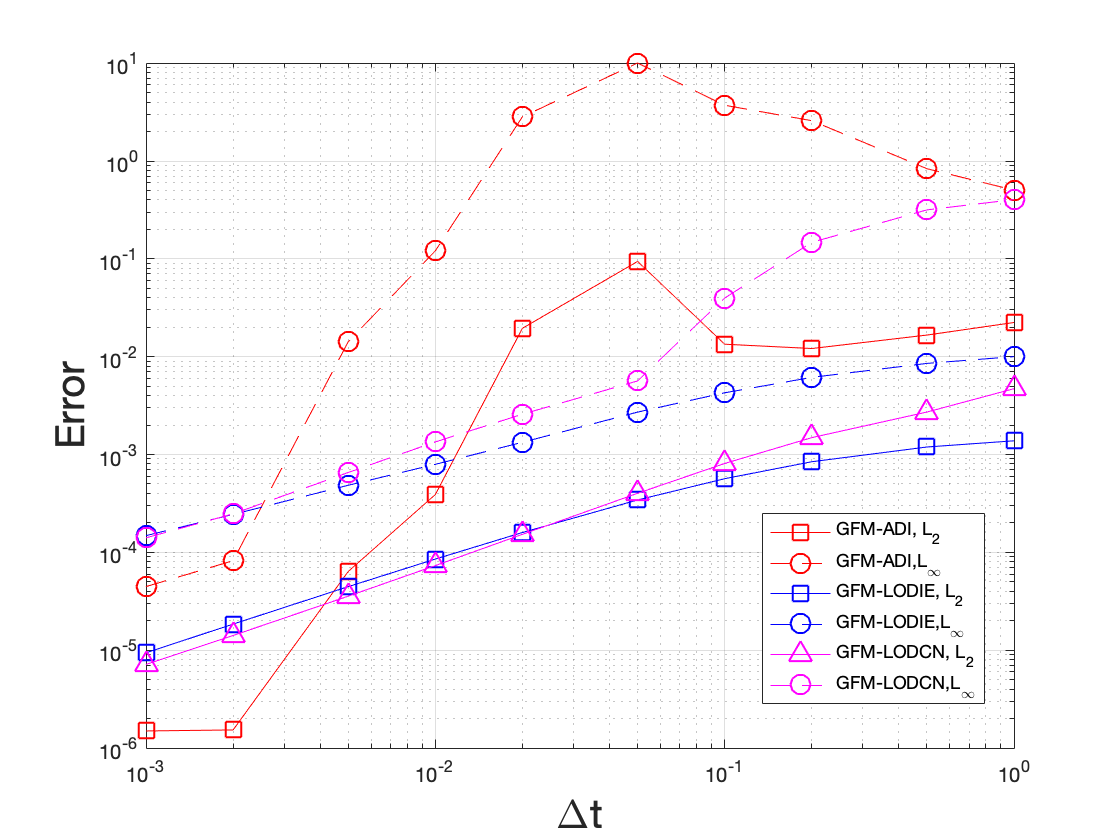
\includegraphics[width=4in]{temp.png}
	\caption{Temporal convergence}
% TODO Have to add ADI methods result 	
\end{figure}
   
\section{Biological applications}

In this section, we focus on exploring the stability and accuracy of GFM-ADI, GFM-LODCN and GFM-LODIE schemes by considering the solvation analysis of real proteins. Even though all of our proposed schemes were found to be stable for the one atom case (Krikwood sphere) for $\Delta t =[0.001,5]$, it is of great interest to see if these schemes are stable for real protein systems. We will compare all three methods in detail for a particular protein system and try to identify the best choice for the time increment $\Delta t $ and the grid spacing $h$ to get the most accurate result within a reasonable amount of time. The optimum $\Delta t$ and $h$ has been used later to calculate the solvation energy of 24 proteins.      

\subsection{Protein Crambin } To validate our proposed schemes with a real protein we have studied the hydrophobic protein Crambin (PDB ID : 1cbn). It is a 46 residue protein homologous to a membrane-active plant toxins \cite{1cbn_paper}. It is found in the seeds of \textit{Crambe abyssinicia} and have local anesthetic activity in a lobster walking leg axon (J. Marquis \cite{1cbn_paper}). We used the MSMS package to generate the molecular surface for this protein using the crystallographic data recored at $130 K$ as reported in \cite{1cbn_paper}. At this step we used the probe radius as $1.4$ the density as $10$ for the MSMS package.
% Table generated by Excel2LaTeX from sheet '1cbn'
\begin{table}[!ht]
\centering
\begin{tabular}{c c c c c }
\hline
%      & \multicolumn{3}{c }{h =1/2}                   \\ \hline
$\Delta t$  & ADI  & GFM-ADI       & GFM-LODCN     & GFM-LODIE     \\ \hline
%0.001 & -302.90138868 & -302.83729044 & -302.03341621 \\ %\hline
%0.005 & -302.90138868 & -302.83729044 & -302.03341621 \\ %\hline
%0.01  & -302.85075766 & -302.68957418 & -301.31096348 \\ %\hline
%0.02  & -302.69227062 & -302.33466174 & -300.06953533 \\ %\hline
%%0.03  & -302.49342491 & -301.93879794 & -298.97743897 \\ \hline
%%0.04  & -302.27488337 & -301.51872505 & -297.97906854 \\ \hline
%0.05  & -302.04538862 & -301.08386563 & -297.04896758 \\ %\hline
%%0.06  & -301.80951214 & -300.64096822 & -296.17267652 \\ \hline
%%0.07  & -301.56994437 & -300.19496277 & -295.34086258 \\ \hline
%%0.08  & -301.32859818 & -299.74929181 & -294.54698251 \\ \hline
%%0.09  & -301.08701698 & -299.30637260 & -293.78618610 \\ \hline
%0.1   & -300.84648128 & -298.86787256 & -293.05472908 \\ %\hline
%0.2   & -298.63624081 & -294.81110682 & -286.88648904 \\ %\hline
%%0.3   & -296.77150162 & -291.23283125 & -282.05981018 \\ \hline
%0.5   & -293.21633440 & -284.83429816 & -274.64462149 \\ %\hline
%0.7   & NaN           & -279.04495504 & -269.01031327 \\ %\hline
%%0.9   & NaN           & -273.75954410 & -264.47533078 \\ \hline
%1     & NaN           & -271.29161057 & -262.50478312 \\ %\hline
%2     & NaN           & -251.54655749 & -248.89416804 \\ %\hline
%%3     & NaN           & -237.49060662 & -240.78175990 \\ \hline
%5     & NaN           & -218.29937773 & -230.91124478 \\\hline
0.001 & -459.5742719854 & -303.00657886   & -303.00154088   & -302.80556740 \\
0.002 & -458.1104685049 & -302.99808443   & -302.98279503   & -302.61375402 \\
0.005 & -452.1116748705 & -302.90138868   & -302.83729044   & -302.03341621   \\
0.01  &    NaN         & -302.85075766   & -302.68957418   & -301.31096348   \\
0.02  &    NaN         & -302.69227062   & -302.33466174   & -300.06953533   \\
0.05  &    NaN          & -302.04538862   & -301.08386563   & -297.04896758   \\
0.1   &    NaN          & -300.84648128   & -298.86787256   & -293.05472908   \\
0.2   &    NaN           & -298.63624081   & -294.81110682   & -286.88648904   \\
0.5   &    NaN          & -293.21633440   & -284.83429816   & -274.64462149   \\
0.7   &   NaN           & NaN             & -279.04495504   & -269.01031327   \\
1     &     NaN         & NaN             & -271.29161057   & -262.50478312   \\
2     &    NaN          & NaN             & -251.54655749   & -248.89416804   \\
5     &    NaN           & NaN             & -218.29937773   & -230.91124478 \\ \hline
\end{tabular}
\caption{Solvation Energy ({\it kcal/mol}) of 1cbn for $h=0.5$ and the ionic strength $I_s= 0.15$}
\label{tab-1cbn}
\end{table}

  For this study at first we reported the solvation energy of 1cbn calculated by all three of our proposed schemes in Table \ref{tab-1cbn}. After calculating electrostatic potential $\phi$, equation (\ref{eq_solvation}) has been discretized further to calculate the solvation energy as, 
 \begin{equation}
 	E_{\rm sol} = \sum_i \sum_j \sum_k Q({x_i,y_j,z_k}) \phi_{RF}(x_i,y_j,z_k)
 \end{equation} 
where $Q$ is the trilinear interpolation of the singular charges $q_i$ at the center of the atoms.  The potential values are obtained by scaling our calculated dimensionless potentials with the constant $0.596163438$ corresponding for the room temperature (300K). In all cases a uniform mesh size $h = 0.5$ and a large stopping time $T$ will be used to ensure that the steady state solution is reached. For the dielectric constant we have used $\epsilon^+=80$ for water as the solvent and $\epsilon ^-=1$ the region in side the protein. The ionic strength has been used as $I_s = 0.15$.
 
Here we tried to identify the value of $\Delta t$ as large as possible without losing the adequate amount accuracy for a real protein like 1cbn. But in Table \ref{tab-1cbn} as we have observed  for $\Delta t > 0.5$, GFM-ADI diverges totally while other two schemes loses significant amount of accuracy. If we consider the solvation energy (around -302 {\it kcal/mol}) for $\Delta t =0.005$ as the most accurate one and compare all other solvation energies in Table \ref{tab-1cbn}, it can be observed that with the increase of $\Delta t$ all three proposed schemes looses accuracy but at a different rate. GFM-ADI scheme is usually more accurate while GFM-LODIE schemes more robust to the larger values of $\Delta t$. The performance of GFM-LODCN is roughly in between the other two schemes in terms of accuracy and stability. To be uniform  with the studies for the other proteins in this paper we have used the optimum value for $\Delta t =0.05$ and $h=0.5$. 
\begin{figure}[!ht]
\begin{center}	
	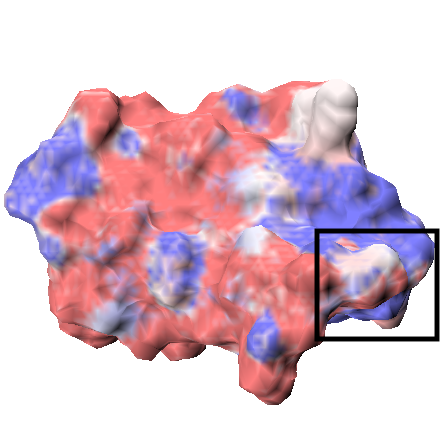
\includegraphics[width=2.1in]{1cbn_gfmadi_front_sq.png}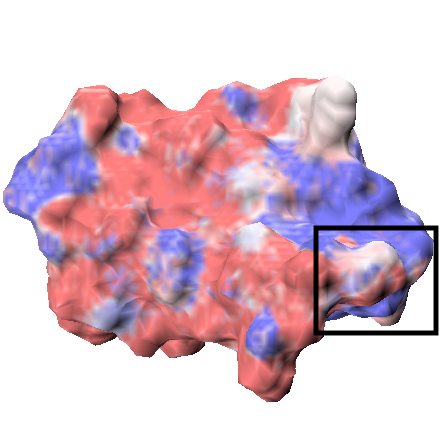
\includegraphics[width=2.1in]{1cbn_gfmlodcn_front_sq.png}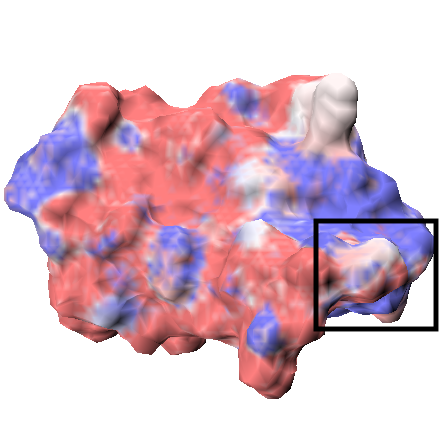
\includegraphics[width=2.1in]{1cbn_gfmlodie_front_sq.png}\\
GFM-ADI front \hskip 0.7in GFM-LODCN front \hskip 0.7in GFM-LODIE front\\
	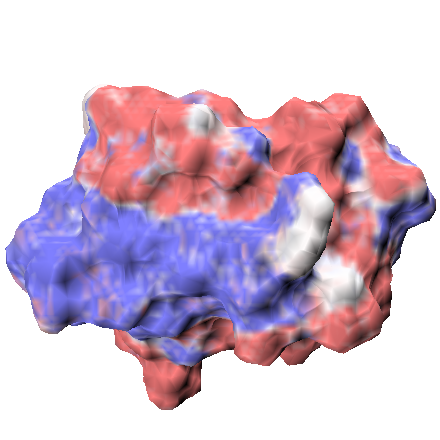
\includegraphics[width=2.1in]{1cbn_gfmlodcn_back.png}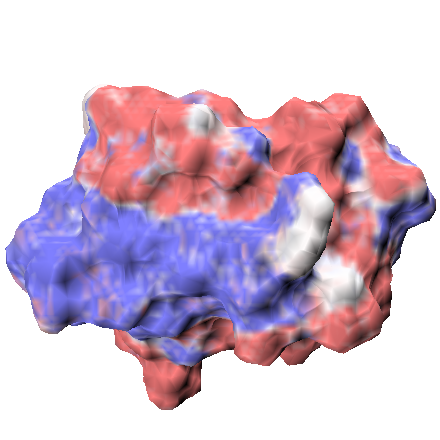
\includegraphics[width=2.1in]{1cbn_gfmlodcn_back.png}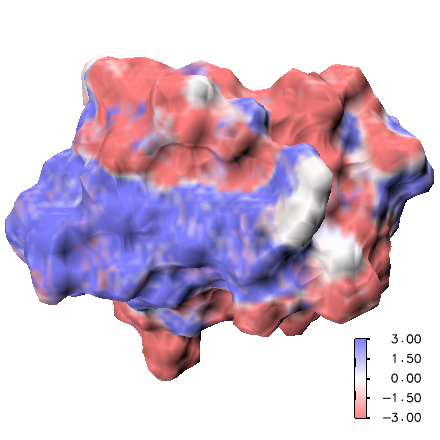
\includegraphics[width=2.1in]{1cbn_gfmlodie_back_scale_1.png}\\
  GFM-ADI back \hskip 0.7in GFM-LODCN back \hskip 0.7in GFM-LODIE back\\
	\caption{Electrostatic potential for 1cbn using $dt = 0.05$ and $h= 0.5$. }
\label{fig_1cbn}
\end{center}
\end{figure}

In Figure \ref{fig_1cbn} we focus on the electrostatic potential on the surface of the protein 1cbn for all three of our prosed schemes.  The difference is not that much noticeable unless we focus in the black squared region of the front side. This shows that, even though there are some differences in solvation energies calculated by the proposed three methods there is no significant difference for the electrostatic potentials for our choice for the optimum values of the parameters.      



\subsection{Solvation energy of 24 proteins}
Next we solved the nonlinear PB equation and computed solvation energy for a collection of 24 proteins as in \cite{Geng2007,Geng2017a}. The dielectric constants , Ionic strength and all other parameters have been set similar to our study for the protein Crambin(1cbn).  
 

\begin{table}[!ht]
\centering
\begin{tabular}{ c c c c c c c c}
\hline
\scriptsize{PDB} & \scriptsize{No. of Atoms}& \scriptsize{rMIB}   &   \scriptsize{ADI}    &  \scriptsize{GFM-ADI}  & \scriptsize{GFM-LODCN} & \scriptsize{GFM-LODIE}\\ \hline
1ajj & 519  & -1139.48 & -1371.10 & -1139.45 & -1139.07 & -1133.06 \\
2erl & 573  & -952.36  & -1165.28 & -952.13  & -951.03  & -945.96  \\
1cbn & 648  & -303.33  & -459.51  & -302.06  & -301.09  & -297.06  \\
1vii & 596  & -902.31  & -1154.67 & -901.78  & -901.36  & -895.15  \\
1fca & 729  & -1204.44 & -1458.16 & -1205.53 & -1205.09 & -1199.33 \\
1bbl & 576  & -988.40  & -1302.49 & -986.15  & -985.72  & -979.60  \\
2pde & 667  & -820.97  & -1018.66 & -819.17  & -819.83  & -813.45  \\
1sh1 & 702  & -753.99  & -999.92  & -751.69  & -751.84  & -745.15  \\
1vjw & 826  & -1241.07 & -1513.17 & -1244.74 & -1243.52 & -1236.67 \\
1uxc & 809  & -1139.25 & -1478.20 & -1138.50 & -1135.22 & -1128.39 \\
1ptq & 795  & -873.32  & -1170.00 & -867.98  & -867.40  & -859.71  \\
1bor & 832  & -853.47  & -1102.40 & -852.49  & -851.24  & -844.68  \\
1fxd & 824  & -3321.39 & -3653.81 & -3321.68 & -3321.34 & -3313.83 \\
1r69 & 997  & -1088.62 & -1419.35 & -1085.45 & -1084.66 & -1076.32 \\
1mbg & 903  & -1353.31 & -1685.70 & -1352.63 & -1351.30 & -1343.68 \\
1bpi & 898  & -1304.37 & -1672.02 & -1301.61 & -1299.86 & -1291.40 \\
1hpt & 858  & -812.49  & -1147.42 & -809.02  & -808.09  & -799.24  \\
451c & 1216 & -1027.21 & -1379.27 & -1023.71 & -1022.61 & -1012.70 \\
1svr & 1435 & -1711.11 & -2257.80 & -1707.87 & -1706.38 & -1693.11 \\
1frd & 1478 & -2862.50 & -3376.35 & -2863.69 & -2863.03 & -2850.42 \\
1a2s & 1272 & -1921.20 & -2292.15 & -1919.28 & -1917.70 & -1907.96 \\
1neq & 1187 & -1731.71 & -2223.08 & -1729.87 & -1728.61 & -1716.47 \\
1a63 & 2065 & -2374.41 & -3149.69 & -2370.80 & -2369.26 & -2350.42 \\
1a7m & 2809 & -2160.34 & -2771.41 & -2155.05 & -2152.48 & -2135.73 \\ \hline
\end{tabular}
\caption{Solvation energies ({\it kcal/mol}) of 24 Proteins considering $\Delta t = 0.001$ for ADI and $\Delta t =0.05$ for GFM-ADI, GFM-LODCN, GFM-LODIE}
\label{tab_24protein}
\end{table}
Solvation energies for all three of our proposed schemes have been compared  with the rMIB and MIB schemes in Table \ref{tab_24protein}. The results from our proposed schemes have been observed to be very close to the results from rMIB and MIB schemes while solving nonlinear PB equation instead of linear PB equation. As we have identified in previous subsections GFM-ADI  appeared to be more accurate than the other two of our proposed schemes and obtained the same level of accuracy as rMIB and MIB schemes. Table \ref{tab_24protein} also confirms that if GFM-ADI fails to converge for any protein then GFM-LODCN or GFM-LOD can also be used since they are more stable and the results are not that much different than GFM-ADI.   
\begin{figure}
	\centering
	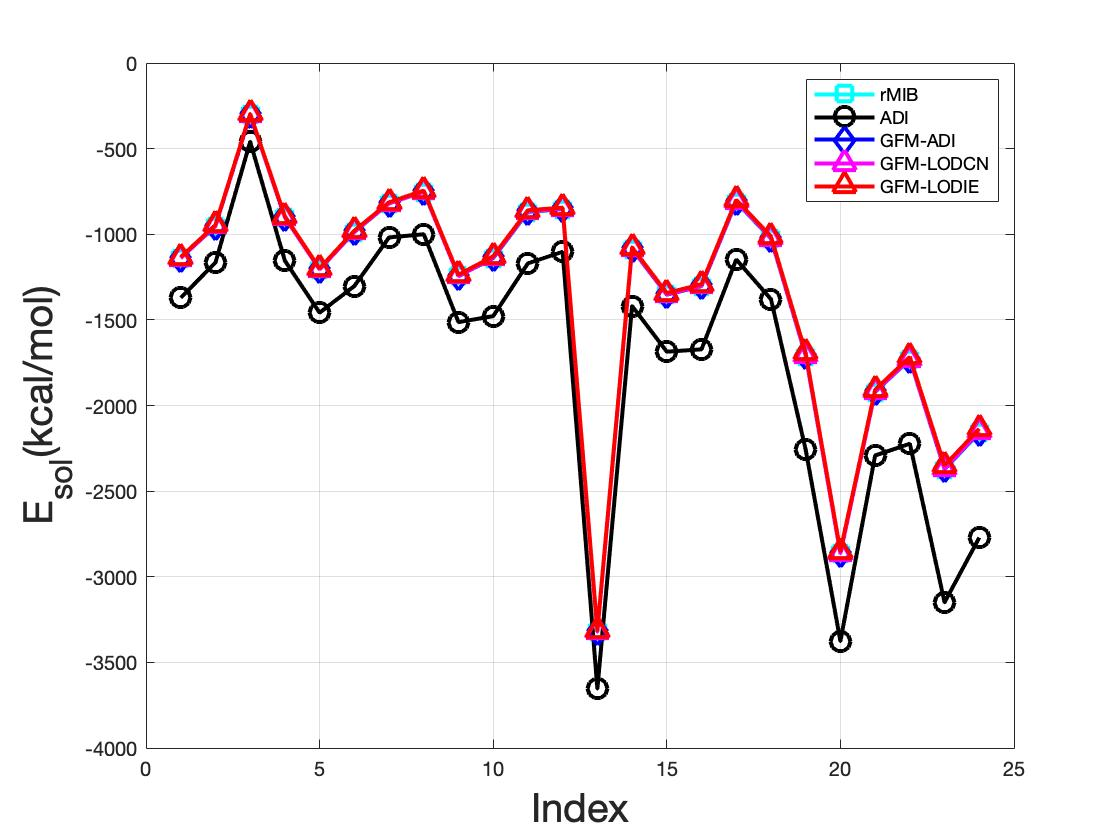
\includegraphics[width=3.2in]{24_energy}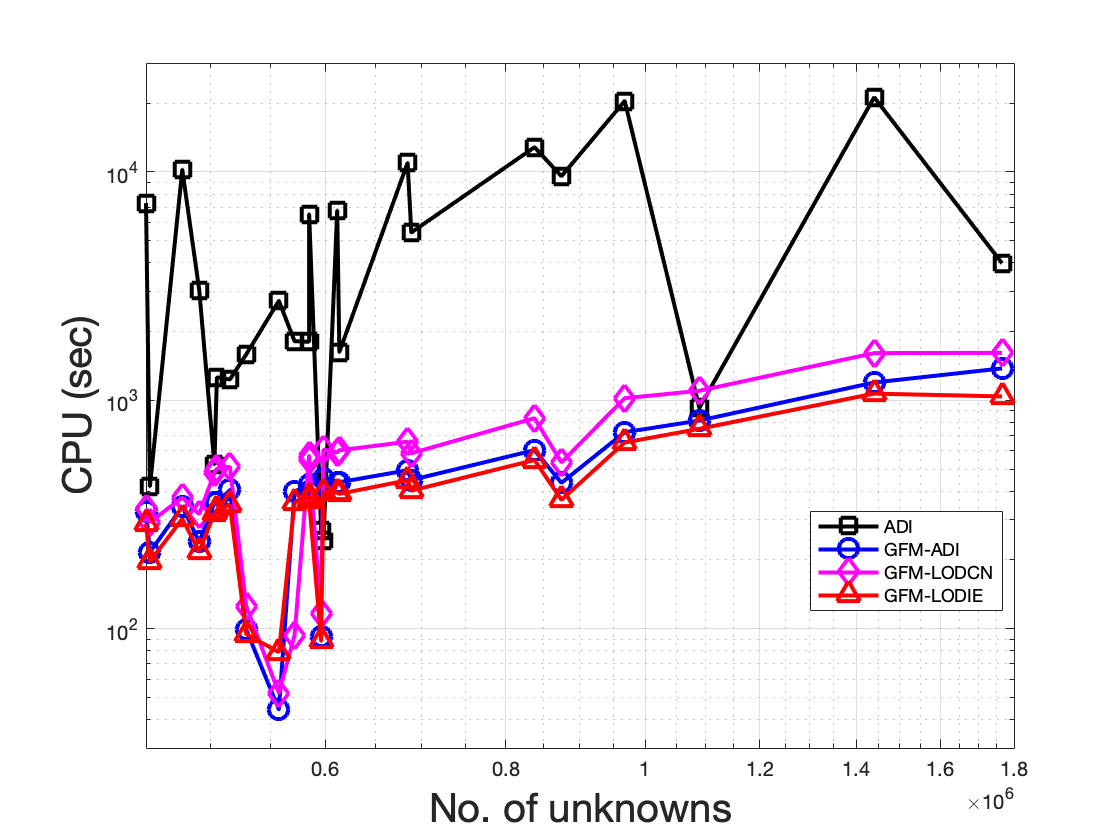
\includegraphics[width=3.2in]{CPU_time}
\caption{Difference in solvation energy(left) and CPU time (right) in solving nonlinear PB eqation for 24 protein. }
\end{figure}

\subsection{Binding energy of 2a9x}

Binding energies play an important role in viral transcription and antiviral drug designs. In particular a better accuracy of the binding energy of the BIV Tat Protein and BIV TAR RNA in HIV viral replication can significantly help in search for the new antiviral drugs that repress the replication by blocking transactivation of viral RNA transcription \cite{Leeper2005}. In this section we will demonstrate the ability of GFM-ADI scheme to compute the binding energy of the BIV Tat Protein and BIV TAR RNA. 

The electrostatic binding free energy can be calculated by the following formula based on the free energy cycle,
\begin{eqnarray}
	E^{\rm AB}_{\rm bind}&=&\Delta G^{\rm AB}_{\rm ele}-\Delta G^{\rm A}_{\rm ele}-\Delta G^{\rm B}_{\rm ele}\label{eq_bind}\nonumber \\
	&=& [E^{\rm AB}_{\rm sol}+E^{\rm AB}_{\rm cou}]-[E^{\rm A}_{\rm sol}+E^{\rm A}_{\rm cou}]-[E^{\rm B}_{\rm sol}+E^{\rm B}_{\rm cou}]
\end{eqnarray}
	
where the free energies of the complex $AB$ and its monomers $A$ and $B$ on the RHS can be calculated using the calculated solvation energies in equation (\ref{eq_Gele}). 
\begin{table}[!ht]
\centering
\begin{tabular}{crrrr}
\hline
$h$ & $E_{\rm sol}^{\rm complex}$ & $E_{\rm sol}^{\rm protein}$ & $E_{\rm sol}^{\rm RNA}$ & $E_{\rm bind}^{\rm complex}$ \\ \hline
\multicolumn{5}{c}{rMIB}  \\ \hline
1   & -5816.38 & -1021.94 & -8893.39 & 383.60 \\
1/2 & -5821.22 & -1025.86 & -8898.54 & 387.84 \\
1/4 & -5823.39 & -1026.27 & -8900.52 & 388.05 \\ \hline
\multicolumn{5}{c}{GFM-ADI}  				  \\ \hline
1   & -5834.10 & -1027.14 & -8915.17 & 392.84 \\
1/2 & -5824.82 & -1025.98 & -8905.59 & 391.38 \\
1/4 & -5841.62 & -1026.40 & -8916.69 & 386.12 \\ \hline
\end{tabular}
\caption{Binding energy of 2a9x}
\label{tab_2a9x}
\end{table}


%    where the calculated solvation energies ($E_{\rm sol}$) will be added with the coulomb energies ($E_{\rm cou}$) to get the free energies ($\Delta G$) for the complex $AB$ and the monomers $A$  and $B$. 

\begin{figure}[!ht]
	\begin{center}
		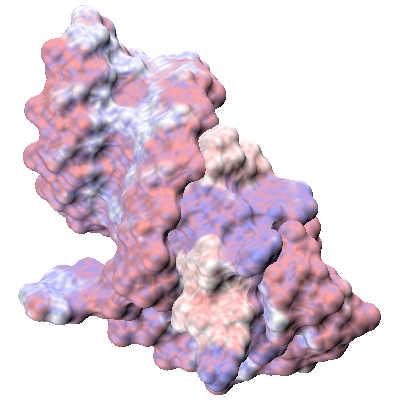
\includegraphics[width=3in]{complex_front.png}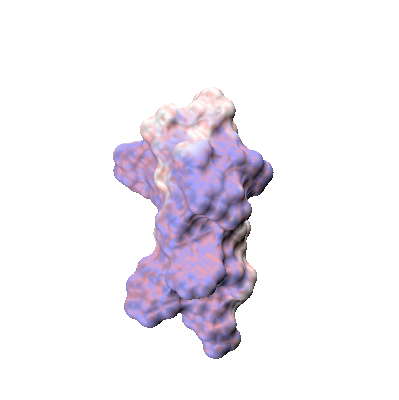
\includegraphics[width=3in]{protein_back.png}\\
		\hskip 0.5in 2a9x complex front\hskip 2.5in 2a9x  protein back\\
		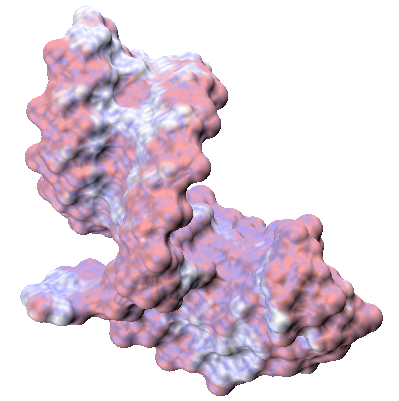
\includegraphics[width=3in]{rna_front.png}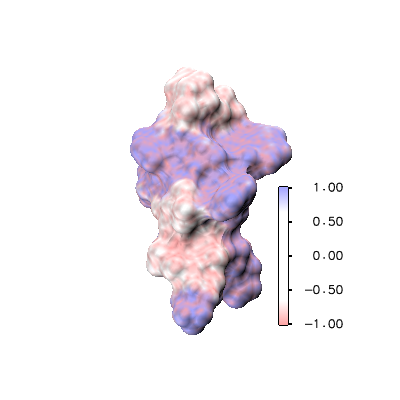
\includegraphics[width=3in]{protein_front_scale_right.png}\\
		\hskip 0.7in 2a9x rna front\hskip 2.8in 2a9x  protein front\\
		\caption{Electrostatic potential for 2a9x using GFM-ADI for $\Delta t = 0.05$ and $h = 0.5$}
	\end{center}
\end{figure}
%todo Have to include the table of binding enrgy

\subsection{Salt effect on the binding affinity}
The nonlinear PB equation is often used to describe the salt effects on the binding of ligands, peptides, and proteins to nucleic acids, membranes, and proteins. In this investigation we have tested the the performance of the proposed GFM-ADI scheme for the evaluation of the salt effect in the protein-protein binding of the complex 1beb and 1emv. Physically, the binding affinity can be quantitatively represented based on the binding-free energies, which reflect the non-specific salt dependence of the formation of macro- molecular complexes. The binding affinity is then calculated as the slope ratio of the salt-dependent binding energy at certain salt strength $I_s$ against the natural logarithm of $I_s$.
The electrostatic binding-free energy can be further split into $E_{\rm cou}(I_s)$'s as the salt-independent parts and $E_{\rm sol}(I_s)$'s as the salt-dependent parts. The variation of the salt-dependent part of the binding-free energy $\Delta E_{\rm bind}(I_s)$ can thus be calculated as the difference in $E_{\rm bind}(I_s)$ for some nonzero salt strength and the zero salt concentration, because the salt independent parts gets simply cancelled. Altogether we have the following formula.\\
\begin{eqnarray}
	\Delta E_{\rm bind}(I_s) &=& E_{\rm bind}(I_s)- E_{\rm bind}(0)\label{eq_del_e_bind} \nonumber\\
						 &=& [E_{\rm sol}^{\rm AB}(I_s)-E_{\rm sol}^{\rm AB}(0)]-[E_{\rm sol}^{\rm A}(I_s)-E_{\rm sol}^{\rm A}(0)]- [E_{\rm sol}^{\rm B}(I_s)-E_{\rm sol}^{\rm A}(0)]\end{eqnarray}
For this study we have used the same model parameters used earlier for 24 proteins. In Figure \ref{fig_salt_effect} we reported the calculated binding free energy with the experimental results.The slope ration or the binding affinity is calculated and reported in Table (\ref{tab_salt_effect}) as in \cite{zhao_pseudo-time-coupled_2011}. The results attained by the Lagrangian formulation linearized PB (LFLPB) model \cite{Zhan_2011} are also given in Table (\ref{tab_salt_effect}) for comparison. For 1beb the binding affinity calculated by GFM-ADI scheme sufficiently close to experimental data and better than LFLPB. For 1emv the results from  GFM-ADI is not as good as those of the LFLPB model but qualitatively it agrees with the experimental observations; that is as the hetero-diemric complex, the binding-free energy increases when the ionic strength is larger. This is probably because the calculation of the binding affinity requires a physical cutoff to obtain two monomers A and B.     	
\begin{table}[!ht]
\begin{tabular}{ccclcrrr}
\hline
\multicolumn{2}{c}{}           & \multicolumn{3}{l}{Charges} & \multicolumn{3}{l}{Slope ratios} \\
Complex                 & PDB  & AB       & A       & B      & Experimental & GFM-ADI & LFLPB   \\ \hline
Lactoglobulin dime(A-B) & 1beb & +26      & +13     & +13    & $-1.62$      & $-1.82$ & $-2.02$ \\ %\hline
E9Dnase-Im9(10)(B-A)    & 1emv & $-3$     & $-8$    & +5     & 2.17         & 0.52    & 2.4     \\ \hline
\end{tabular}
\caption{Comparison of binding affinities of the protein complexes 1emv and 1beb}
\label{tab_salt_effect}
\end{table}



\begin{figure}[!ht]
\begin{center}
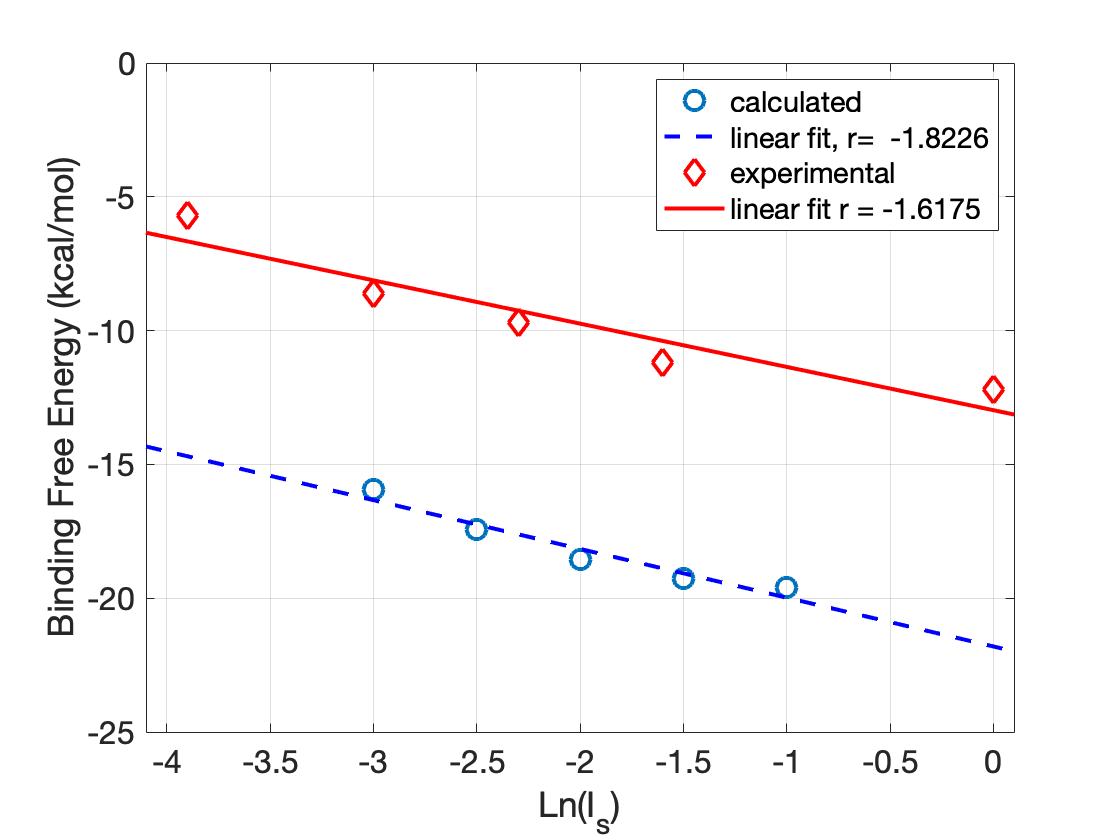
\includegraphics[width =3.2in]{1beb_Tend50_TTol_neg4}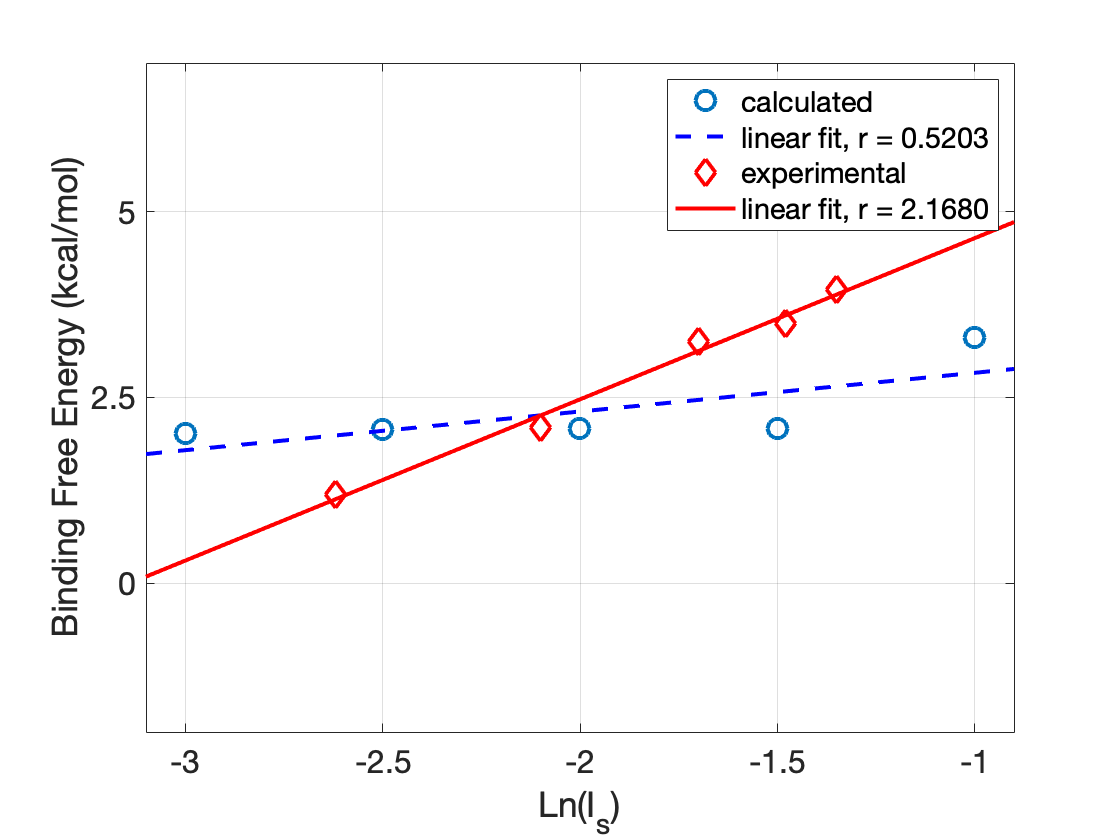
\includegraphics[width =3.2in]{1emv_Tend50_TTol_neg4}\\
1beb \hskip 2.7in 1emv
\end{center}
\caption{The salt dependence of the binding affinities}
\label{fig_salt_effect}
\end{figure}
 

%% -----------------------------Chapter 7 ---------------------------------------
\chapter{CONCLUSIONS}
\label{chap: conclusions}
The pseudo-transient methods and regularization methods are popular methods to solve nonlinear PBE. Even though these two types were successful in circumventing different challenges to solve PBE, each one of them was lacking the advantages of the other one. When we tried to combine them we faced a new challenge due to  the new jump conditions being nonzero. This forced us to find a way to apply interface treatments. The MIB method \cite{Geng2007,Chen2011,Yu2007,ZHAO2004,ZHOU2006,ZHOU2006_high,YU2007_3D} was a great choice for this type of interface treatments but it would have ruined the tridiagonal structure of the finite difference operator matrix of the 1D equations like (\ref{GFM-ADI}) (\ref{GFM-ADI2}) and (\ref{GFM-ADI3}) in all of our proposed methods. Having tridiagonal structure for these three equations are very important since we have to solve all three of them at each time step. So for small time step size, it would take unreasonably long time for the whole system to reach the equilibrium state to produce the solution.   

So we considered the GFM method \cite{Liu2000} for $L=1$ which uses a three point stencil keeping the tridiagonal structure for the 1D equations in our proposed methods. But the original GFM method requires the jump conditions to be in axial directions while the regularized PBE has its jump condition in the normal direction. It motivated us to modify the original GFM  method to able to use the normal direction jump condition by considering approximate jump conditions like (\ref{eq:m-gfm1}) and (\ref{eq:m-gfm2}). 

In comparison with the existing pseudo-transient approaches the GFM-ADI proposed in this dissertation is much more stable than ADI in \cite{Geng2013_Fully}. This makes GFM-ADI a very practical method, while the ADI method is impractical by requiring too small time step size. In some sense, the GFM-ADI method is even better than LOD methods in \cite{Wilson2016}. Although LOD methods are unconditionally stable, energies are inaccurate for large time steps. GFM-LODCN and GFMLOD are also producing more accurate results than its predecessor the LOD methods in \cite{Wilson2016} leaving an option for the cases when GFM-ADI fails to converge. 

In future we have a plan to take the advantage of the simplicity of these proposed schemes to the other areas of molecular biophysics like the problem of computing the electrostatic field and forces for molecular dynamic simulations as in \cite{GENG_WEI2011}. 
 

%% ---------------------------- Reference ---------------------------------------
%% Suggestion: Jabref is a nice free software for references which is compatible with Goodschalor cite function.
\addcontentsline{toc}{chapter}{REFERENCES}
\renewcommand{\bibname}{REFERENCES}
\begin{singlespace}
\bibliography{bibl}
\bibliographystyle{abbrv}
\label{bib}
\end{singlespace}

%%%%%%%%%%%%%%%%%%APPENDIX%%%%%%%%%%%%%%%%%%%%%%
\addcontentsline{toc}{chapter}{APPENDIX}
\appendix

\lipsum








\end{body}
\end{document}
